\chapter{束流模拟程序的优化和性能测试} \label{chap:Performance}
随着加速器束流流强的增大,为了对束流进行精确的模拟和研究,我们需要模拟的粒子数目增加了几个量级。
在这种趋势下,束流模拟软件的效率至关重要。
本文之前在第\ref{chap:Code}章介绍了束流模拟程序在GPU和CPU上的并行实现,
接下来在本章中,首先小节\ref{section:PIC_performance}将对PIC算法在多种计算平台的性能测试进行介绍。
之后,第 \ref{section:Symplectic_performance}节将对Symplectic算法的GPU并行性能进行了测试。

\section{PIC程序性能}             \label{section:PIC_performance}
我们使用了多种计算平台对并行PIC程序的性能进行调优和测试~\cite{tiwari2015Titan,wells2016Summit,he2018Cori}:
\begin{itemize}
  \item 单GPU - GTX1060
  \item GPU集群 - Titan
  \item GPU集群 - SummitDev
  \item CPU集群 - Cori Knight Landing
\end{itemize}

Titan是一台GPU/CPU混合架构的超级计算机,位于美国橡树岭国家实验室(ORNL),
它使用的是由NVIDIA提供的Tesla计算卡和AMD提供的Opteron处理器~\cite{TitanURL}。
SummitDev是同样位于ORNL,是下一代超级计算机Summit的早期测试平台,每个SummitDev节点都有2个IBM POWER8 CPU和4个NVIDIA Tesla P100 GPU~\cite{SummitURL}。
Cori Knight Landing(KNL)是Cori的新计算平台,位于美国国家能源研究科学计算中心(NERSC)。KNL基于Intel众核架构(MIC),每个节点有68个内核和一个AVX-512矢量协处理器~\cite{KnlURL}。

使用单GPU和不同集群的测试综合性地给出了不同计算机架构上PIC代码性能评估。
接下来,如我们之前在第~\ref{section:PIC_GPU_Poisson}节中讨论的,我们首先比较了泊松方程求解在域分解模式和复制模式下的性能。
然后,我们再介绍在各个计算平台上运行的PIC代码的性能结果。

\subsection{泊松方程求解}
\label{section:PIC_performance_Poisson}

\subsubsection{单GPU测试}
首先,我们在单GPU上对域分解模式进行了测试,并统计了每一部分所花费的时间。测试的格点数为$64 \times 64 \times 64$,每部分所花费的时间如表\ref{tab:1GPU_Poisson},表中的单位为秒,每部分占比如图\ref{fig:1GPU_Poisson}。

\begin{table}[!htbp]
    \centering
    \footnotesize% fontsize
    \setlength{\tabcolsep}{4pt}% column separation
    \renewcommand{\arraystretch}{1.2}%row space
    \begin{tabular}{lc}
        \hline\hline
        从CPU拷贝到GPU    & 1.306     \\
        \hline
        从GPU拷贝到CPU    & 2.979     \\
        \hline
        FFT计算                       & 0.487     \\
        \hline
        转置和通讯                  & 3.772     \\
        \hline
        总计                              & 8.544    \\
        \hline\hline
    \end{tabular}
    \caption{单GPU域分解模式解泊松方程耗时}
    \label{tab:1GPU_Poisson}
\end{table}

\begin{figure}[!htb]
    \centering
    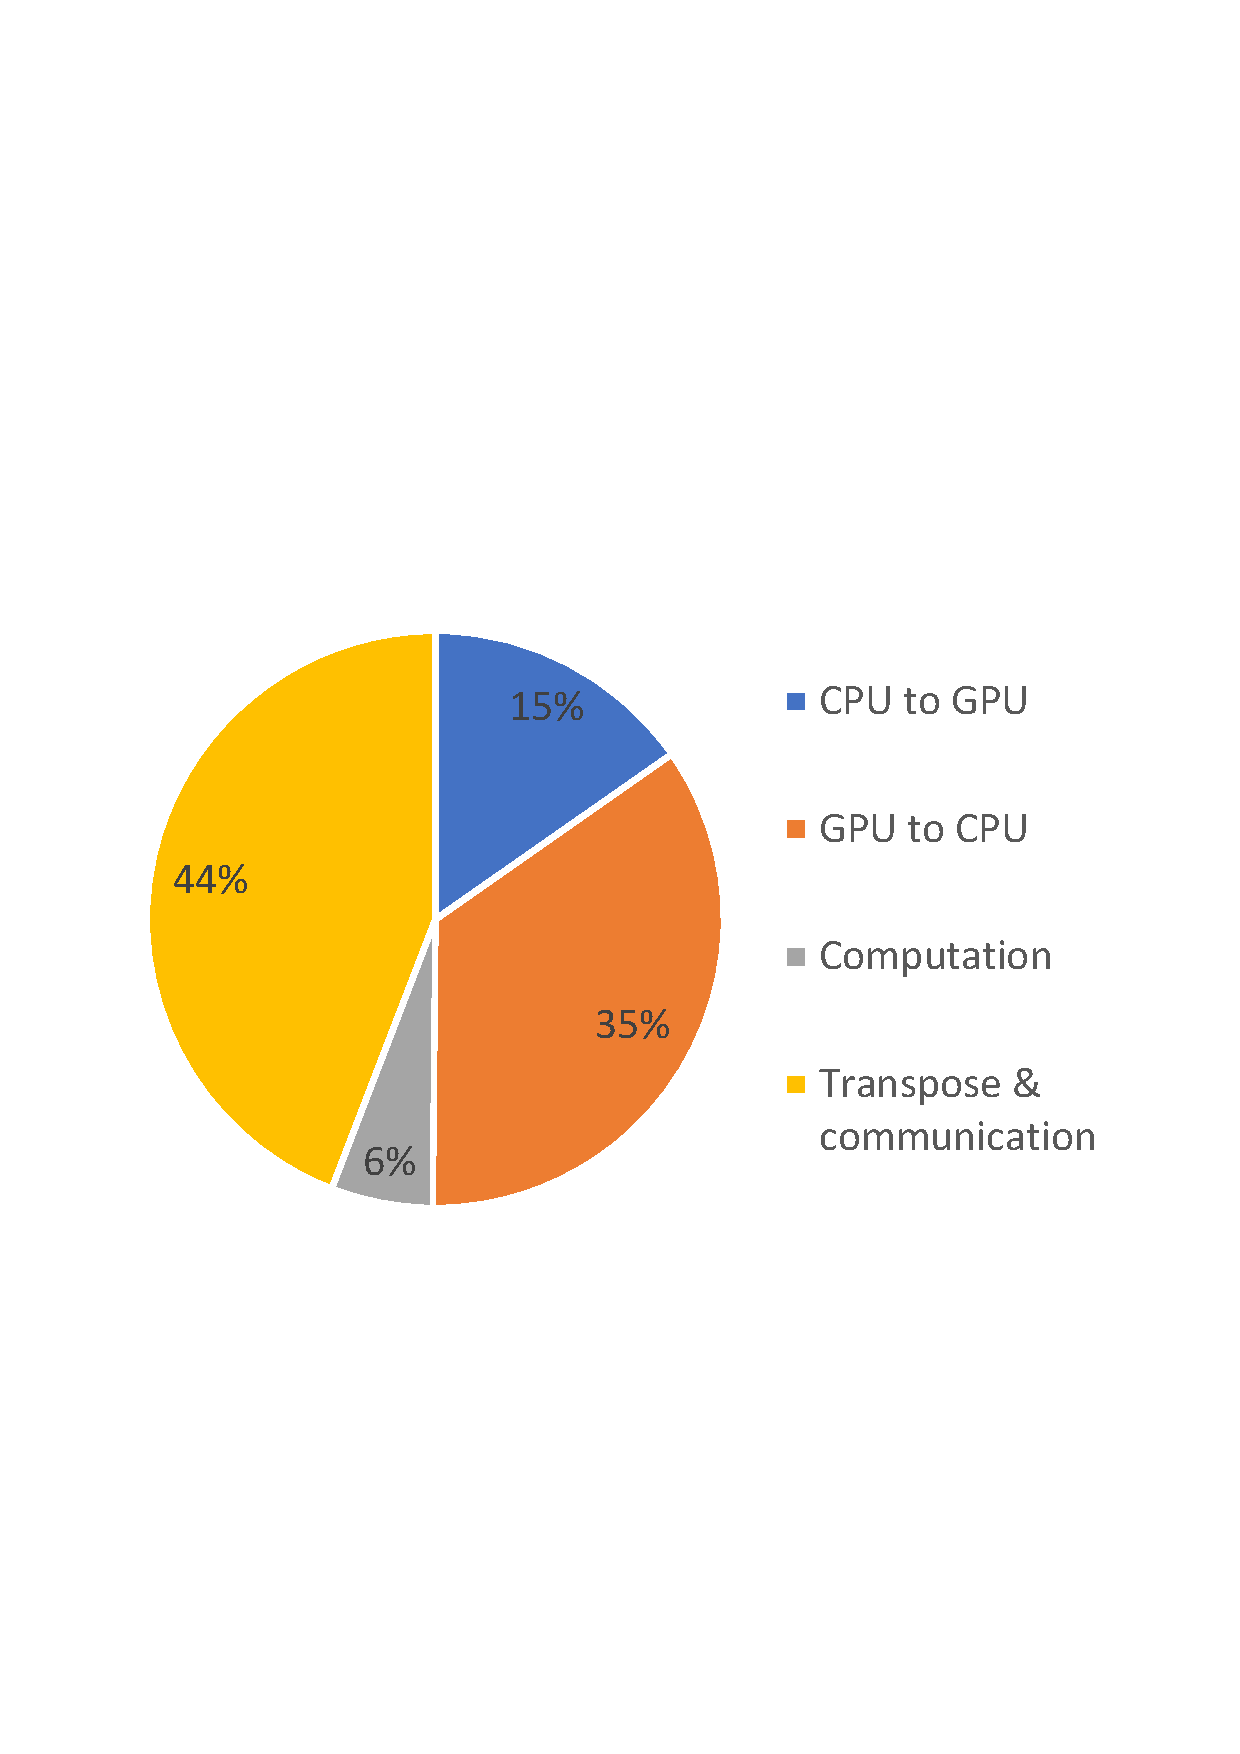
\includegraphics[width=0.55\textwidth]{Img/domain_decomposition_1GPU.pdf}
    \caption{单GPU域分解模式解泊松方程各部分耗时占比}\label{fig:1GPU_Poisson}
\end{figure}

可以看出,FFT计算所花的时间为0.487秒,相比于额外增加的数据拷贝时间1.306 + 4.627 = 4.933秒,其占比非常小,仅仅占总时间的6\%。

多GPU的一种方式是使用同一节点内使用多个GPU,因为节点内的总线宽度限制,数据拷贝时间并不会随着使用GPU数目的增加而明显减少。而复制模式只需要花费FFT计算的时间,因为FFT计算花费的时间0.487秒远小于数据拷贝的时间4.933秒,所以即使在理想情况下使用N个GPU时FFT计算的时间减少到原来的1/N,域分解模式的总时间依然是比复制模式要大。

多GPU的另一种使用跨节点的多个GPU,即每个节点有1个GPU,通过使用多个节点来使用多个GPU,这也是目前超级计算机TITAN的运行模式。
总线宽度会随着节点数增加而增加,所以数据拷贝时间会下降,假设其下降为线性的,
即在N个节点上运行的话拷贝数据时间只有原来的1/N,则总时间将会是 $4.933/N+0.487/N$,
如果我们想要取得优于复制模式的速度,即 $4.933/N+0.487/N<0.487$, GPU数目必须大于11。
类似的,如果我们想要取得两倍的速度,GPU数目必须大于22。然而,这个计算忽略了CPU和CPU之间的通讯时间,
一般来说,节点间的通讯时间随着节点数目增加而增加,因此我们很难取得理想情况的加速比。

下面,我们分别对节点内多GPU和跨节点GPU进行测试。

\subsubsection{单节点多GPU测试}
在同一节点中,我们进行了格点数为$64 \times 64 \times 64$的多GPU测试,
表\ref{tab:2GPU_Poisson}是各个部分所花费的时间,以及和单GPU时的对比。
可以看出,双GPU的总时间更大了,由8.544秒增加到了9.537秒。
其中,FFT计算的时间有0.487秒减少到了0.249秒,几乎减少了一半,
证明了多GPU对于减少纯FFT计算时间是确实有效的;对于数据拷贝时间,双GPU略有减少,
大概减少了三分之一;总时间中增加的部分来源于通讯的时间,几乎增加了一倍。
\begin{table}[!htbp]
    \centering
    \footnotesize% fontsize
    \setlength{\tabcolsep}{4pt}% column separation
    \renewcommand{\arraystretch}{1.2}%row space
    \begin{tabular}{lcc}
        \hline\hline
                          & 1GPU    & 2GPU   \\
        \hline\hline
        从CPU拷贝到GPU    & 1.306   & 0.817  \\
        \hline
        从GPU拷贝到CPU    & 2.979   & 1.991  \\
        \hline
        FFT计算           & 0.487   & 0.249  \\
        \hline
        转置和通讯        & 3.772   & 6.480  \\
        \hline
        总计              & 8.544   & 9.537  \\
        \hline\hline
    \end{tabular}
    \caption{单节点双GPU域分解模式解泊松方程}
    \label{tab:2GPU_Poisson}
\end{table}

\subsubsection{跨节点多GPU测试}
我们使用超级计算机Titan测试了域分解模式下的求解解泊松方程在跨节点多GPU上的效率。
使用常用的$64 \times 64 \times 64$个格点,域分解模式下解泊松方程所花费的时间随GPU个数的变化如图\ref{fig:TITAN_GPU_Poisson64}所示,图中蓝线为总时间,各个柱代表各个部分所花费的时间,图中不清楚部分可以参考表\ref{tab:TITAN_GPU_Poisson64}。

可以看出,程序总耗时随着GPU数目增加而逐渐减少,并在32个GPU的时候到达最小值,随后开始逐渐增加。其中,拷贝数据所花费的时间基本随着GPU的数目线性减少;而通讯所花费的时间先随着GPU数目增加而逐渐减少,到达极值后又开始逐渐增加,此时通讯时间占程序所花费的时间的绝大部分;FFT计算所花费的时间随着GPU数目的增加而逐渐减少,但是FFT计算占总时间的百分比很小。

\begin{figure}[!htb]
  \centering
  \begin{tabular}{|l|l|}
    \multicolumn{2}{c}{
    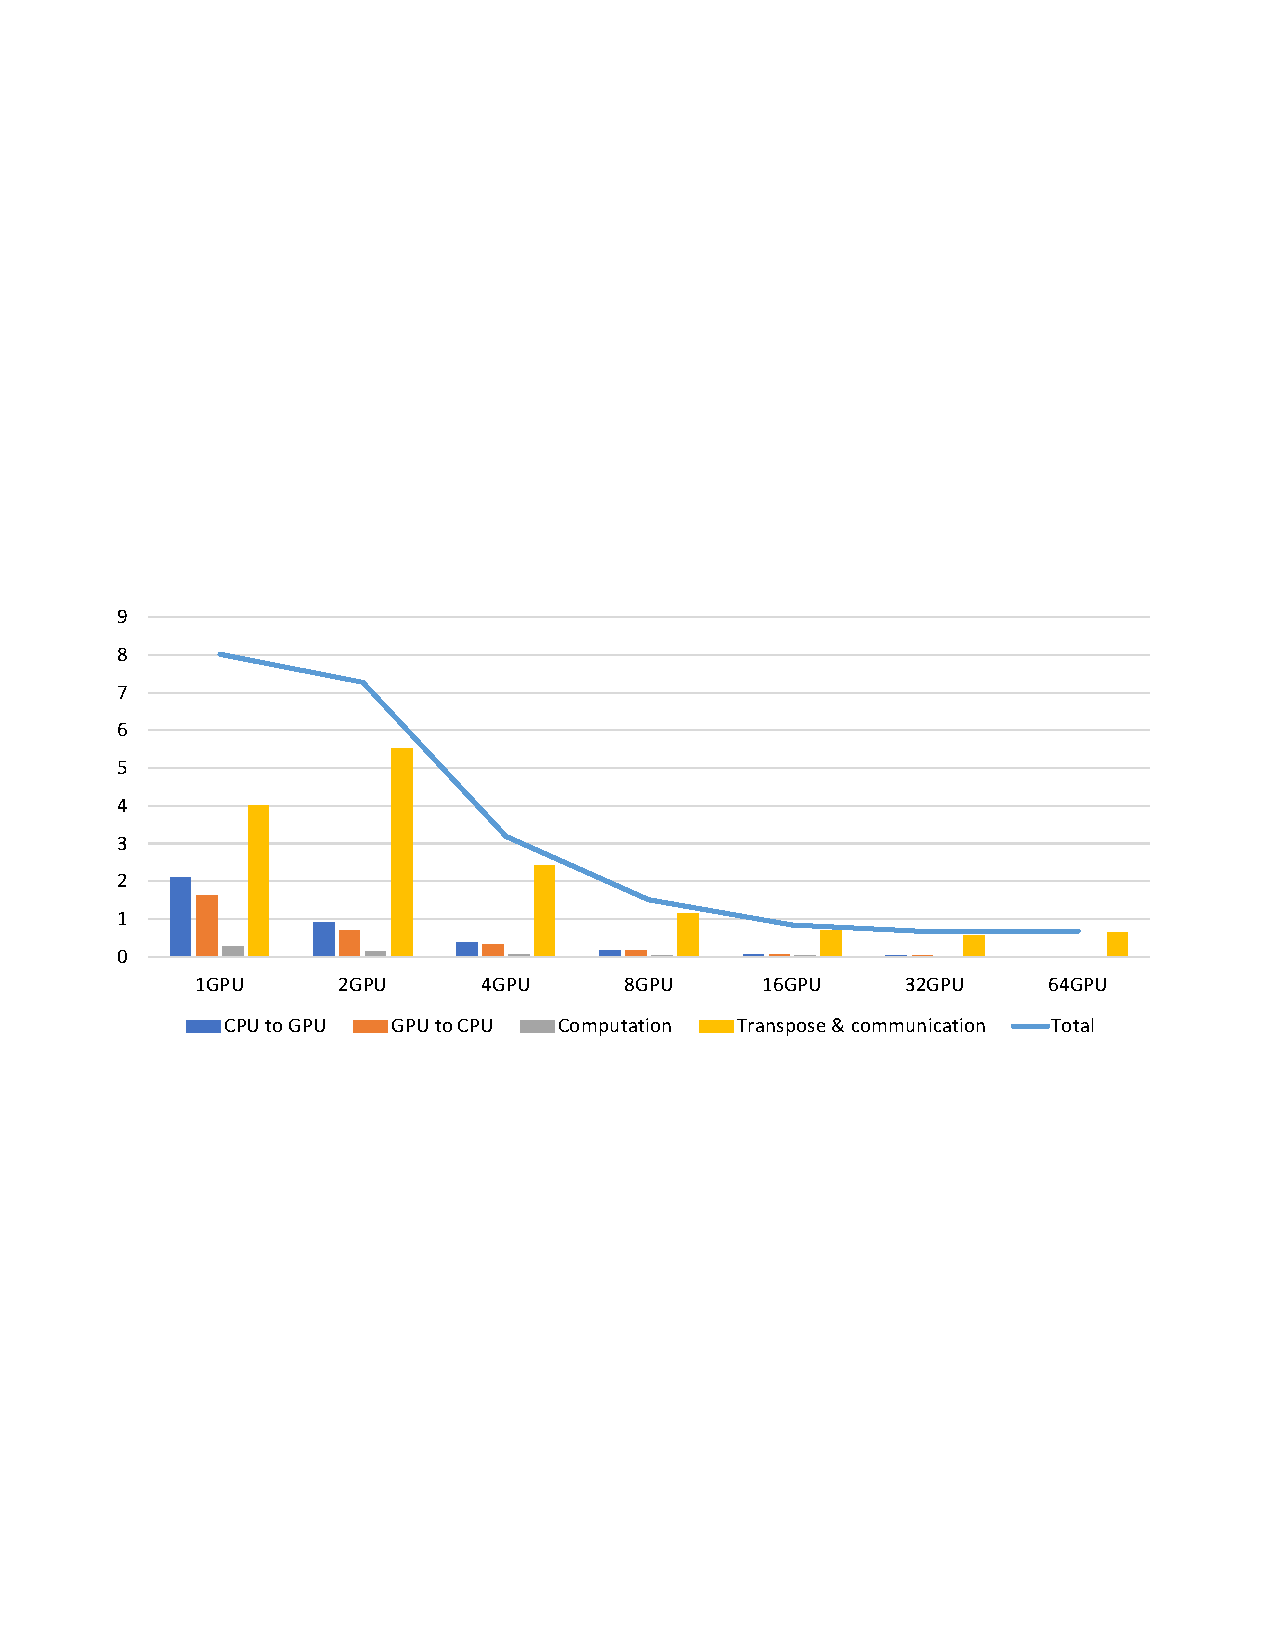
\includegraphics[width=0.9\textwidth]{Img/domain_decomposition_Titan64.pdf}} \\
  \end{tabular}
  \caption{$64 \times 64 \times 64$格点下,跨节点多~GPU~域分解模式解泊松方程时间随~GPU~个数的变化}
  \label{fig:TITAN_GPU_Poisson64}
\end{figure}

\begin{table}
  \centering
  \begin{tabular}{|l|c|c|c|c|c|c|c|}
    \hline
    GPU数目	    &1	    &2	    &4	    &8 	    &16	    &32  	&64   \\
    \hline
    CPU to GPU	&2.111	&0.922	&0.390	&0.158	&0.061	&0.031	&0.0155 \\
    GPU to CPU	&1.618	&0.694	&0.314	&0.167	&0.066	&0.033	&0.0158 \\
    FFT计算  	    &0.266	&0.136	&0.069	&0.039	&0.024	&0.017	&0.0150 \\
    转置和通讯	&4.020	&5.521	&2.415	&1.146	&0.691	&0.572	&0.6320 \\
    总计	        &8.015	&7.273	&3.188	&1.51	&0.842	&0.653	&0.6783 \\
    \hline
  \end{tabular}
  \caption{$64 \times 64 \times 64$格点下,跨节点多GPU 域分解模式解泊松方程各部分所用时间}
  \label{tab:TITAN_GPU_Poisson64}
\end{table}

我们也测试了格点数目更大的情况,格点数目越多,所需要的计算量越大。当格点数为$128 \times 128 \times 128$时,程序在不同的GPU数目下消耗的时间如图\ref{fig:TITAN_GPU_Poisson128}和表\ref{tab:TITAN_GPU_Poisson128}所示,其整体的趋势和$64 \times 64 \times 64$时类似,因为更大的计算量,其总时间在使用128个GPU时到达最小值。

\begin{figure}[!htb]
  \centering
  \begin{tabular}{|l|l|}
    \multicolumn{2}{c}{
    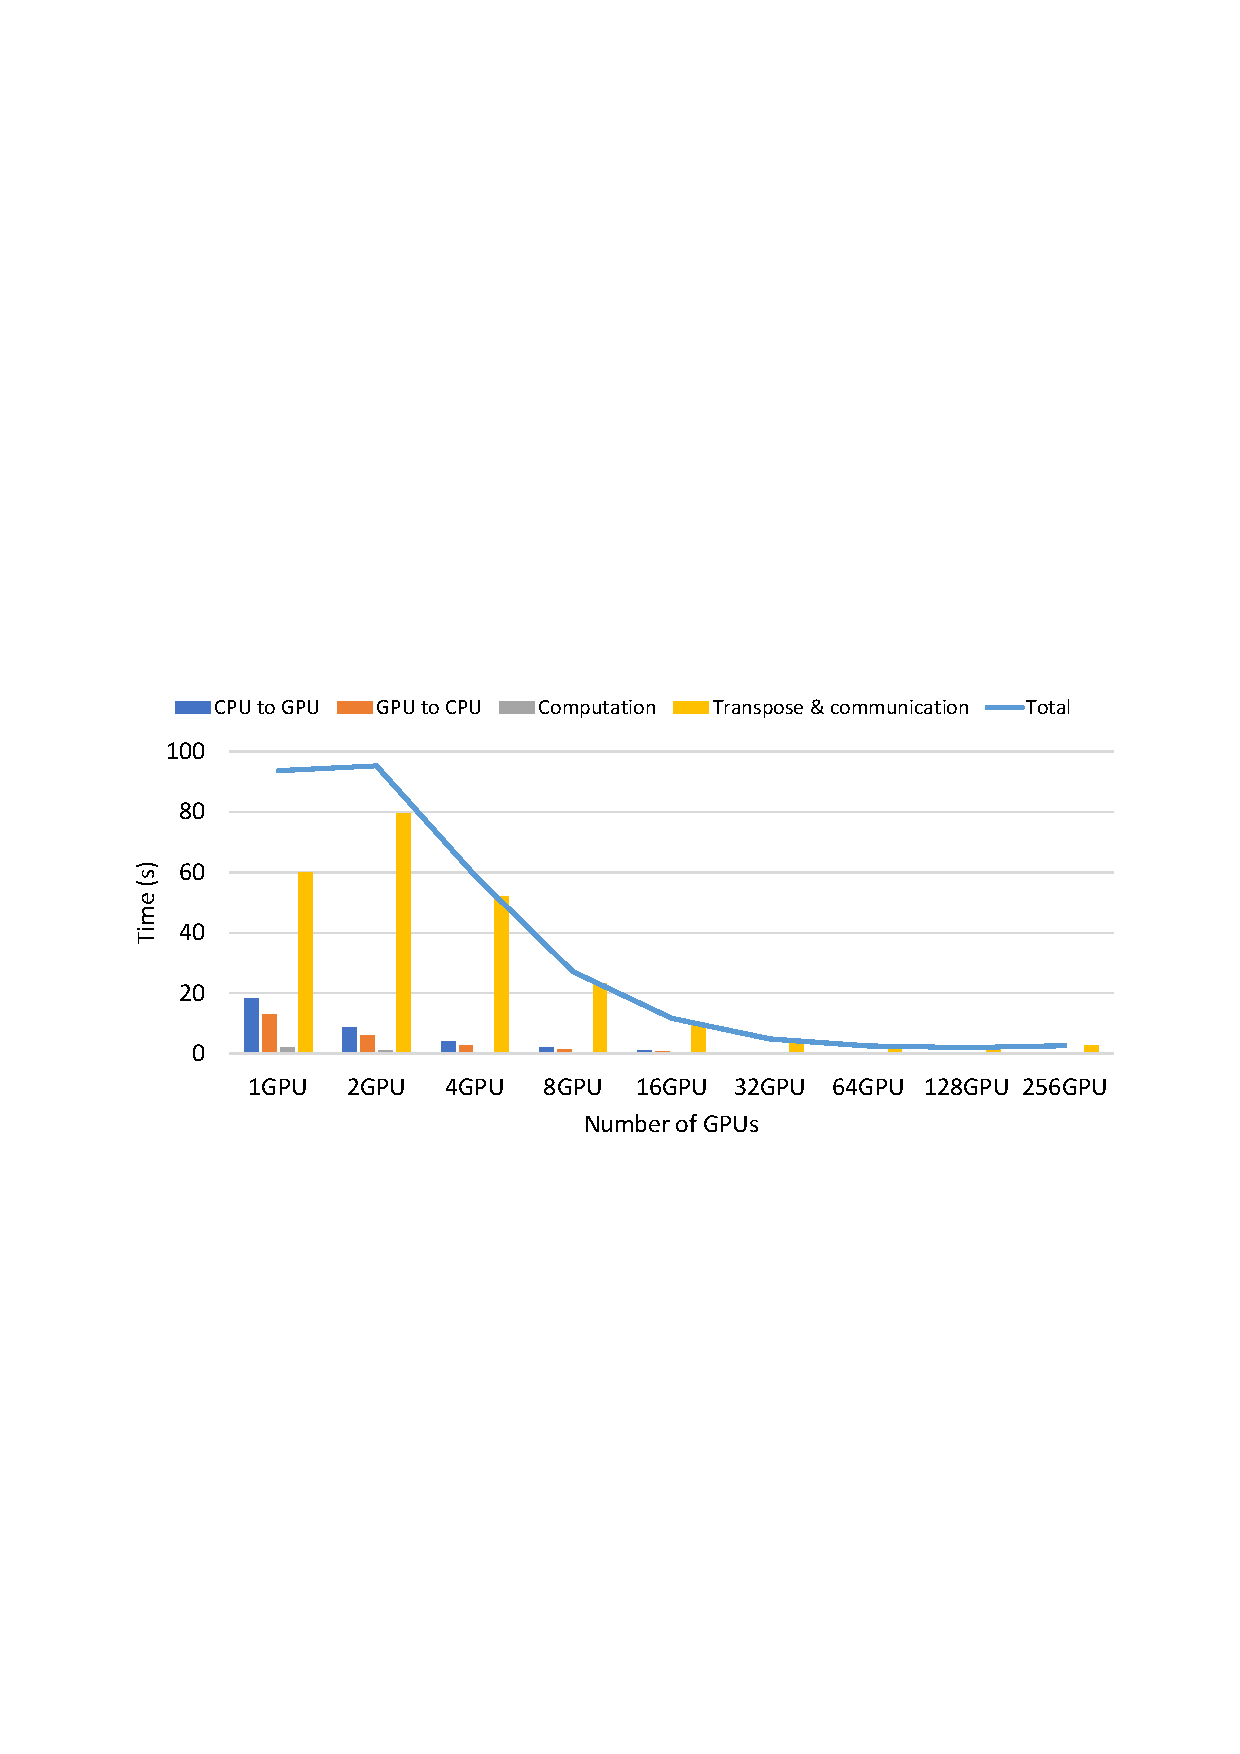
\includegraphics[width=0.9\textwidth]{Img/domain_decomposition_Titan128.pdf}} \\
  \end{tabular}
  \caption{$128 \times 128 \times 128$格点下,跨节点多~GPU~域分解模式解泊松方程时间随~GPU~个数的变化}
  \label{fig:TITAN_GPU_Poisson128}
\end{figure}

\begin{table}
  \centering
  \begin{tabular}{|>{\small}l|c|c|c|c|c|c|c|c|c|}
    \hline
    GPU数目	    &1	    &2	    &4	    &8 	    &16	    &32  	&64     &128	&256   \\
    \hline
    CPU to GPU	&18.29	&8.687	&3.946	&2.023	&0.953	&0.404	&0.148	&0.064	&0.033 \\
    GPU to CPU	&13.11	&6.15	&2.618	&1.463	&0.795	&0.368	&0.139	&0.07	&0.036 \\
    FFT计算  	    &2.185	&1.034	&0.522	&0.266	&0.138	&0.071	&0.036	&0.021	&0.017 \\
    转置和通讯	&59.99	&79.34	&51.85	&23.30	&9.797	&4.041	&2.237	&1.859	&2.506 \\
    总计	        &93.58	&95.21	&58.94	&27.05	&11.68	&4.884	&2.56	&2.014	&2.592\\
    \hline
  \end{tabular}
  \caption{$128 \times 128 \times 128$格点下,跨节点多GPU域分解模式解泊松方程各部分所用时间}
  \label{tab:TITAN_GPU_Poisson128}
\end{table}

在$64 \times 64 \times 64$和$128 \times 128 \times 128$两种情况下,总时间开始都随着GPU数目增加而减小,然后到达最小值,随后由于通讯所需要的时间变大,总时间也随之变大。
然而,无论是使用$64 \times 64 \times 64$个格点还是$128 \times 128 \times 128$个格点,总时间的最小值都大于只是用一个GPU的纯计算时间。
\subsubsection{小结}
通过上面对于“域分解模式”的实现和测试,可以看出程序运行速度主要受限于CPU和GPU之间数据拷贝的速度与CPU和CPU之间的通讯速度。
如果GPU带宽足够大,或者以后能够实现GPU与GPU之间的直接通讯的话,“域分解模式”可以作为一个可行的方案。
但是在目前,与“复制模式”相比,“域分解模式”由于其额外的数据拷贝和通讯开销,并不能通过减少运算量来达到提高速度的目的。
所以我们在程序中以及在下文中都使用“复制模式”(除非另加说明),即使所有的GPU都同时运行同样的程序。

\subsection{单GPU性能-GTX1060}      \label{section:PIC_Performance_GTX1060}
在测试了泊松方程求解器之后,我们通过对比CPU程序和单个GPU程序的运行速度,来得到GPU程序的加速比。
测试使用的格点数为~ $64 \times 64 \times 64$,加速比等于CPU程序耗时除以GPU程序耗时。
图\ref{fig:PIC_speedup_1GPU}和表\ref{tab:PIC_speedup_1GPU}是粒子数从16k到1.6m时CPU程序和GPU程序各部分耗时以及加速比。
可以看出,程序总耗时的加速比大约有40,程序各个部分的加速比有很大不同。

其中,橙色柱行代表求解泊松方程,其加速比大约是64,而且并不随粒子数目的变化而变化。
事实上,求解泊松方程的计算量主要和格点数相关,而此次测试中我们都是用同样的格点数,
因此其耗时和加速比基本不变,之后我们会比较在不同格点数情况下求解泊松方程的加速比变化。
灰色柱行代表推动粒子的加速比,其随着粒子数目增加而变大,在粒子数较大时取得超过了70的加速比。
浅蓝色和深蓝色柱行分别是权重插值和粒子信息输出的加速比,其中GPU的权重插值部分包括了粒子排序运算,
而且由于其运算的不规则性,加速比较低;而粒子信息输出部分也包含了束团参数的计算,这部分加速比较低是因为输出带宽的限制。


\begin{figure}[!htb]
  \centering
  \begin{tabular}{|l|l|}
    \multicolumn{2}{c}{
    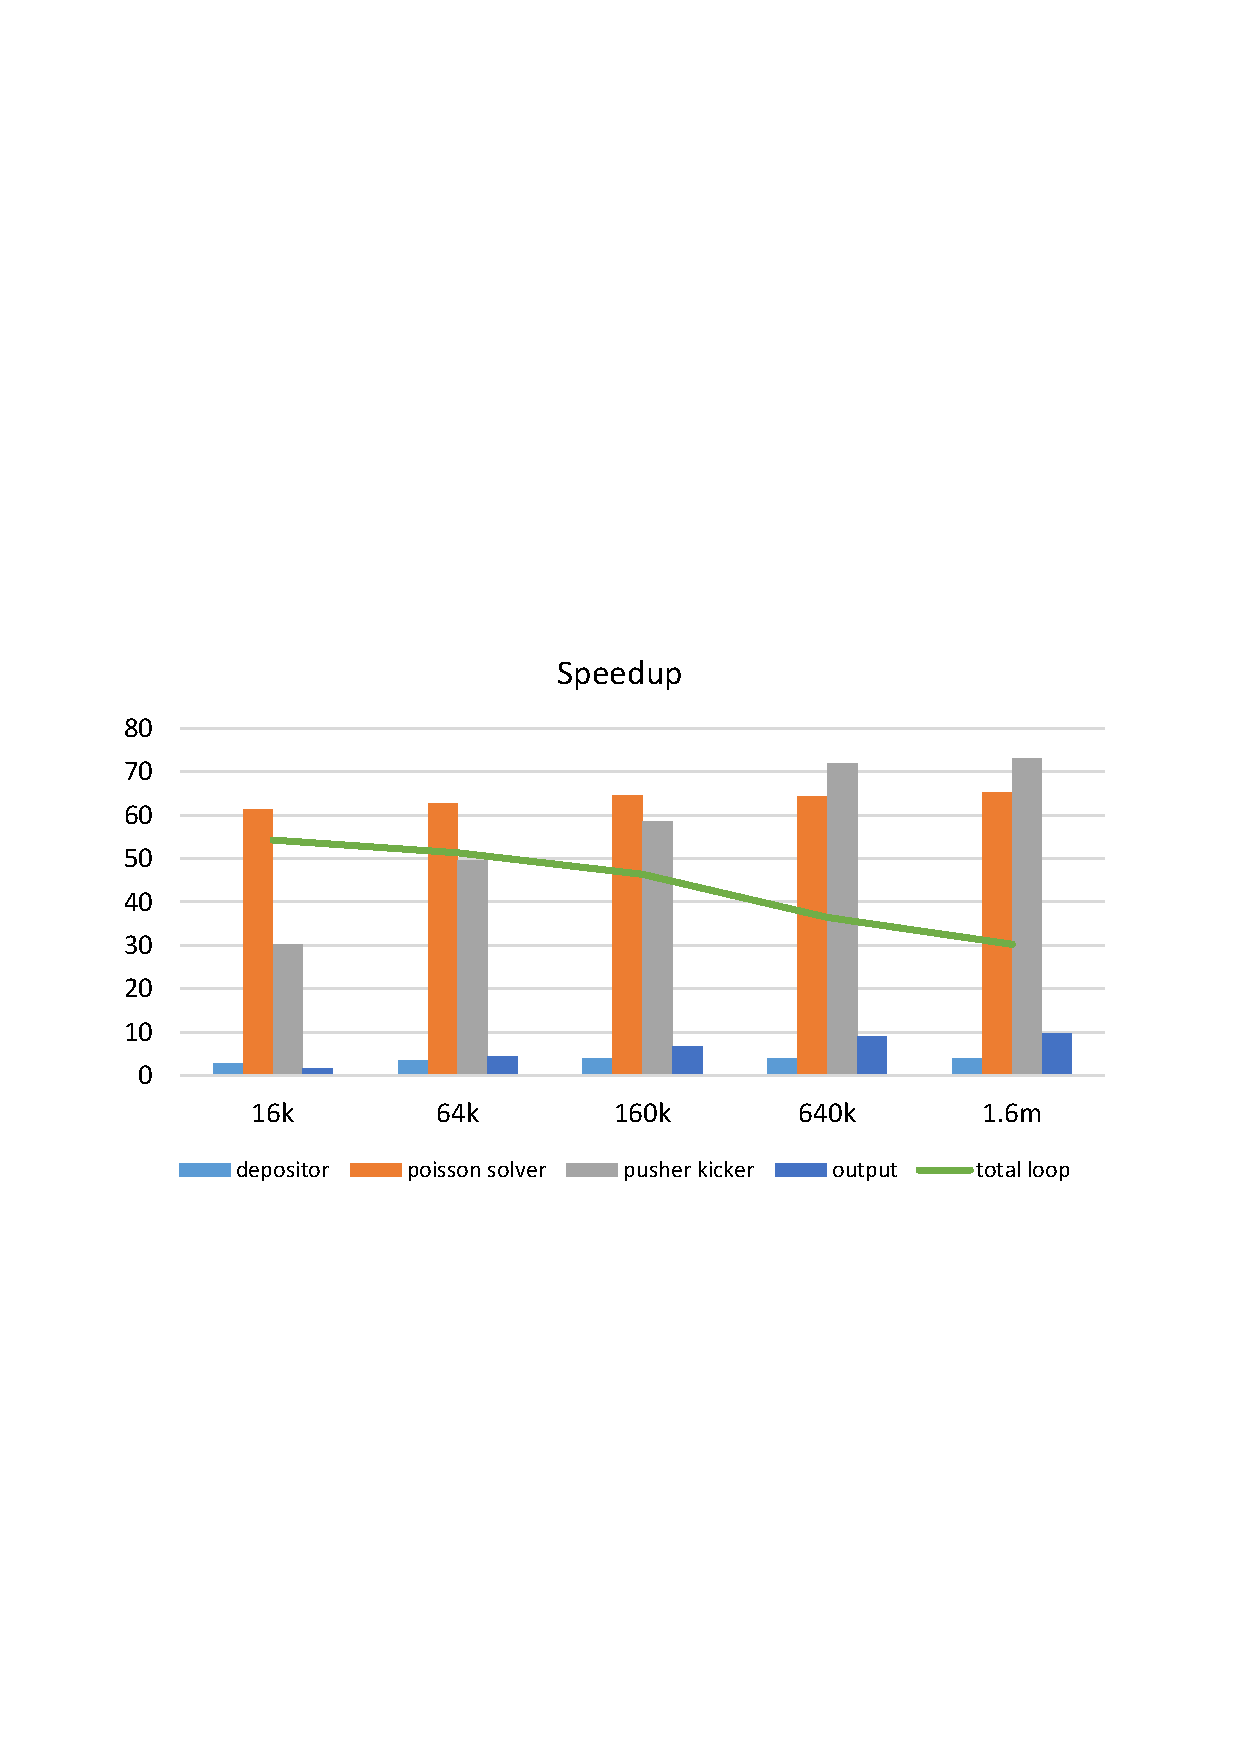
\includegraphics[width=0.9\textwidth]{Img/PIC_speedup_1GPU.pdf}} \\
  \end{tabular}
  \caption{PIC程序在单GPU上的加速比}
  \label{fig:PIC_speedup_1GPU}
\end{figure}

\begin{table}
  \centering
  \begin{tabular}{|l|r|r|r|}
    \hline
    16k                      &    CPU(s)      &     GPU(s)    &  Speedup    \\
    \hline
    depositor (include sort) &    0.16888     &     0.05874   &  2.875043   \\
    Poisson solver           &    26.13173    &     0.42511   &  61.47051   \\
    pusher kicker            &    0.53748	  &     0.01781	  &  30.17855   \\
    output                   &    0.01977     &     0.01149   &  1.720627   \\
    total loop               &    27.78216    &     0.51199   &  54.26309   \\
    \hline
    64k                      &    CPU(s)      &     GPU(s)    &  Speedup    \\
    \hline
    depositor (include sort) &    0.3897      &     0.10847   &  3.592698   \\
    Poisson solver           &    26.08269    &     0.41554   &  62.76818   \\
    pusher kicker            &    2.00422	  &     0.04032	  &  49.70784   \\
    output                   &    0.0641      &     0.01433   &  4.473133   \\
    total loop               &    29.54123    &     0.57598   &  51.28864   \\
    \hline
    160k                     &    CPU(s)      &     GPU(s)    &  Speedup    \\
    \hline
    depositor (include sort) &    0.82705     &     0.20731   &  3.989436   \\
    Poisson solver           &    25.9208     &     0.40208   &  64.46677   \\
    pusher kicker            &    4.88644	  &     0.08343	  &  58.56934   \\
    output                   &    0.15477     &     0.02316   &  6.682642   \\
    total loop               &    32.94187    &     0.71      &  46.397     \\
    \hline
    640k                     &    CPU(s)      &     GPU(s)    &  Speedup    \\
    \hline
    depositor (include sort) &    2.79413     &     0.71529   &  3.90629    \\
    Poisson solver           &    25.72129    &     0.40045   &  64.23097   \\
    pusher kicker            &    22.48269	  &     0.31207	  &  72.04374   \\
    output                   &    0.62289     &     0.06931   &  8.987015   \\
    total loop               &    53.51193    &     1.46745   &  36.46593   \\
    \hline
    1.6m                     &    CPU(s)      &     GPU(s)    &  Speedup    \\
    \hline
    depositor (include sort) &    6.7528      &     1.73779   &  3.885855   \\
    Poisson solver           &    26.03071    &     0.39894   &  65.24969   \\
    pusher kicker            &    56.05512	  &     0.76562	  &  73.21533   \\
    output                   &    1.56528     &     0.16288   &  9.61002    \\
    total loop               &    90.40391    &     2.99053   &  30.23006   \\
    \hline
  \end{tabular}
  \caption{PIC程序在单GPU上的加速比}
  \label{tab:PIC_speedup_1GPU}
\end{table}

权重插值和粒子信息输出的加速比较低,从而拉低了整体的加速比。整体的加速比随着粒子数的增加而逐渐变小,其原因是当粒子数目较小时的时候,求解泊松方程所占得比重较大,从而整体加速比较大;而当粒子数目变大的时候,权重插值所占的时间比重变大,因而整体加速比随之变小。程序各部分耗时在不同粒子数所占比重如图\ref{fig:PIC_speedup_1GPU_percentage}所示。

\begin{figure}[!htb]
    \centering
    \begin{subfigure}[b]{0.75\textwidth}
        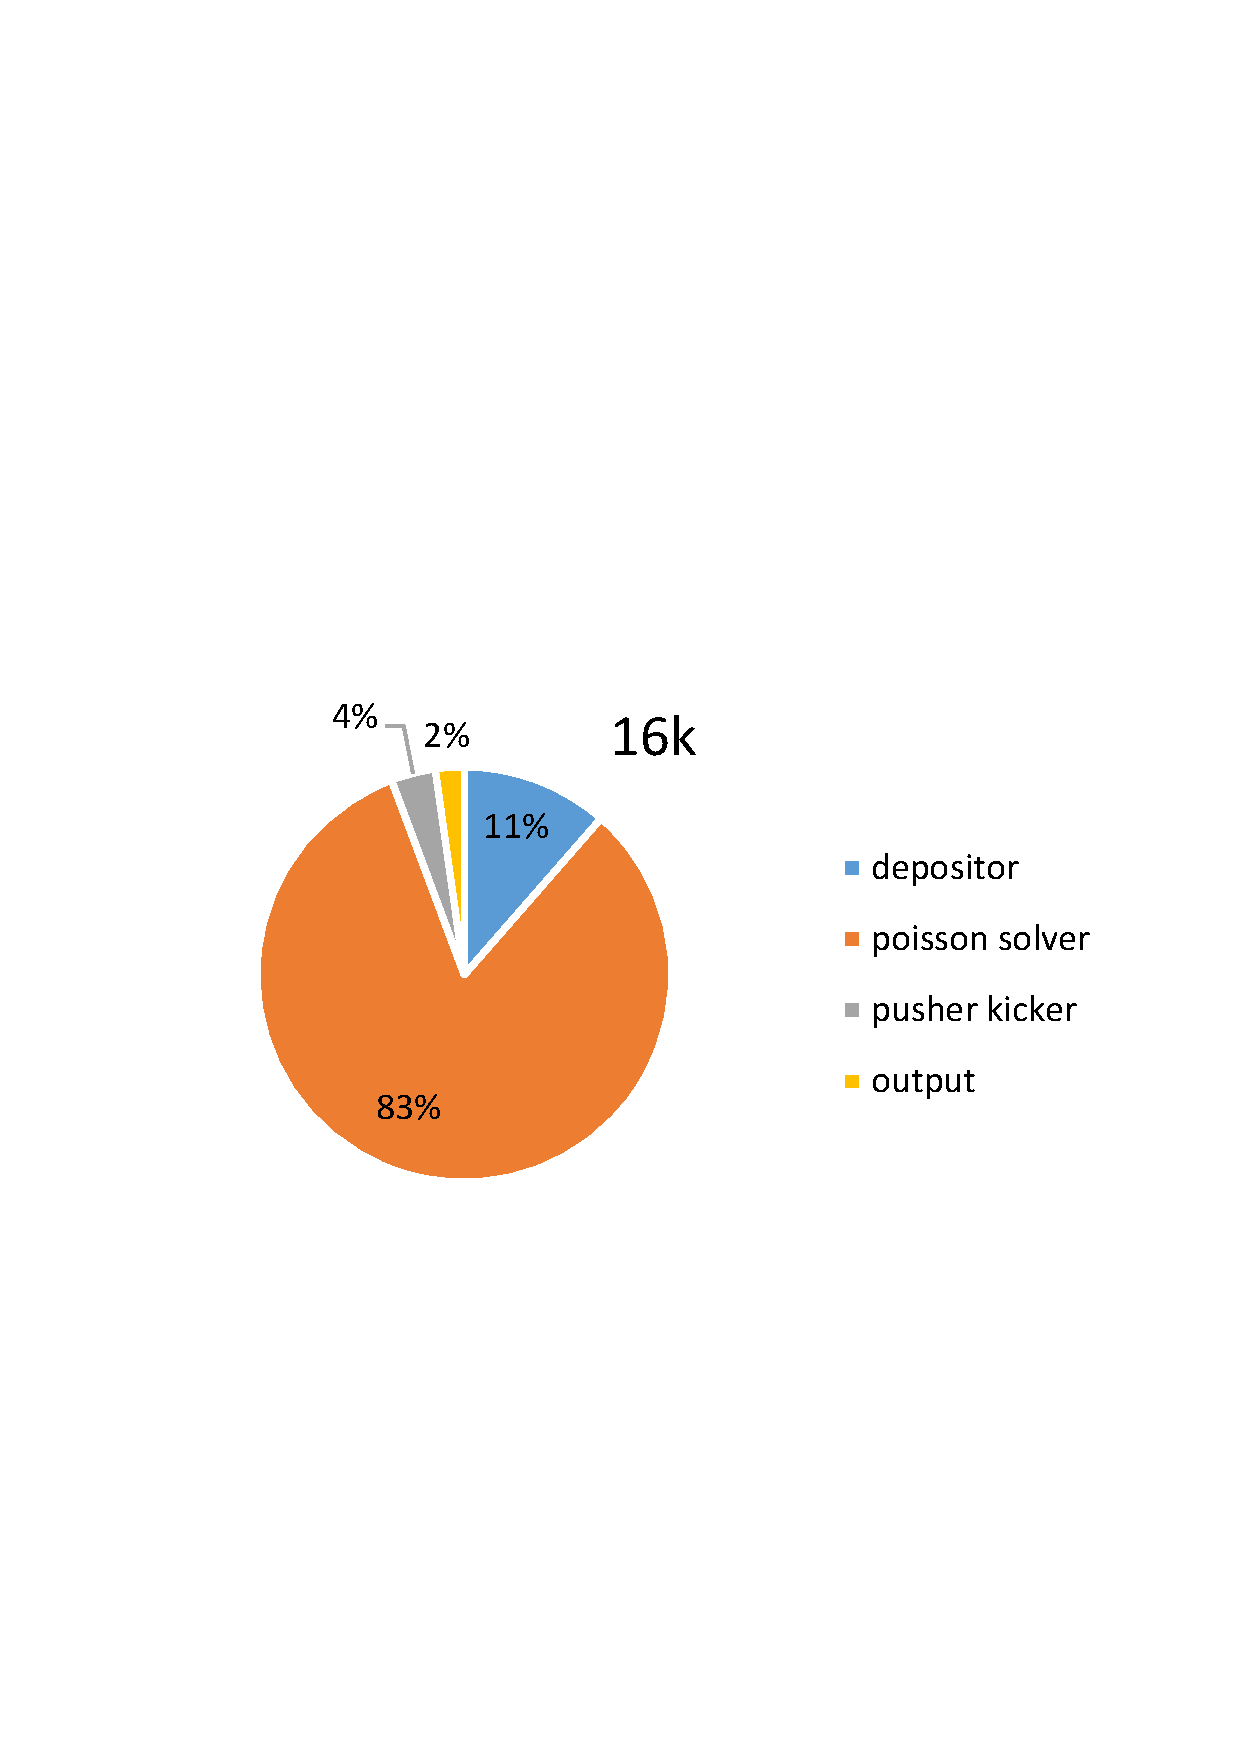
\includegraphics[width=\textwidth]{Img/PIC_speedup_1GPU_percentage1.pdf}
        %\caption{}
    \end{subfigure}
    \quad
    \begin{subfigure}[b]{0.75\textwidth}
        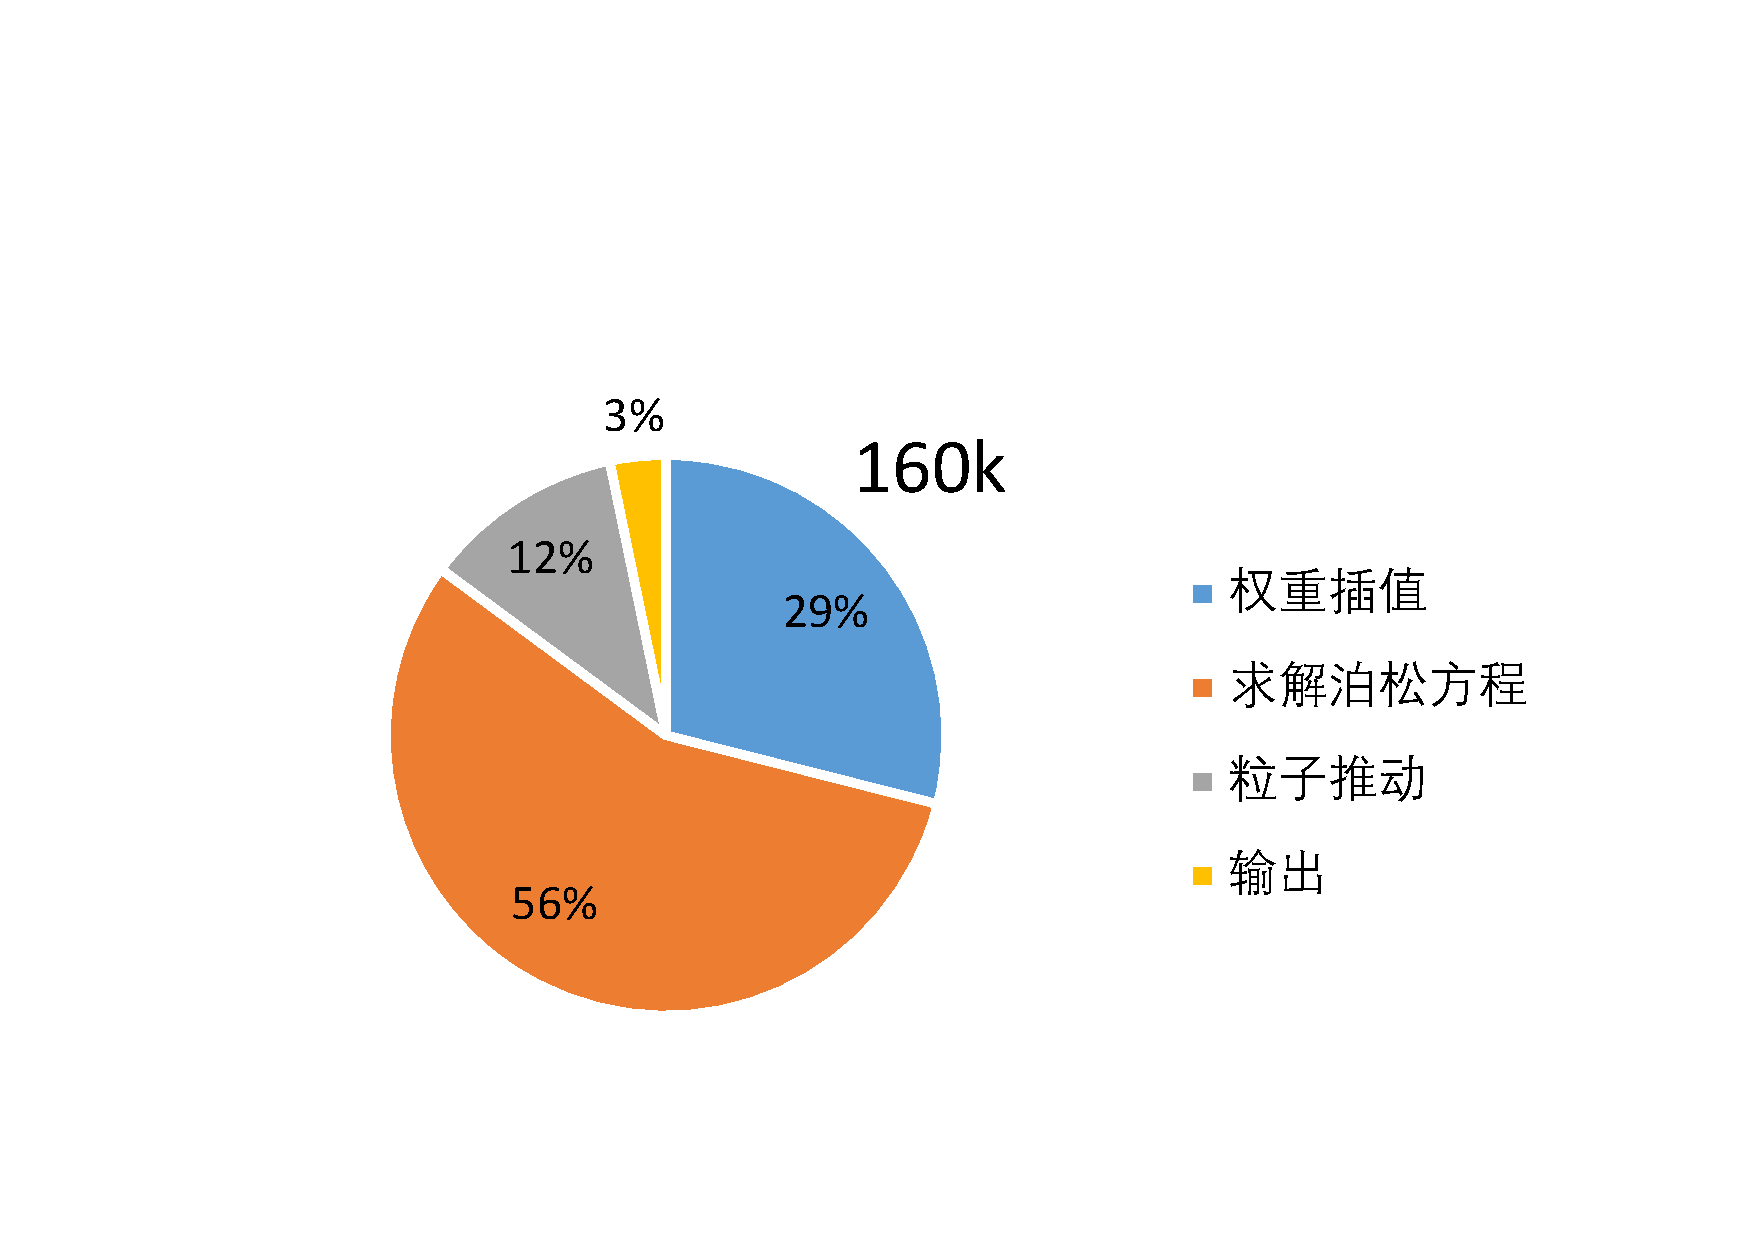
\includegraphics[width=\textwidth]{Img/PIC_speedup_1GPU_percentage2.pdf}
        %\caption{}
    \end{subfigure}
    \quad
    \begin{subfigure}[b]{0.75\textwidth}
        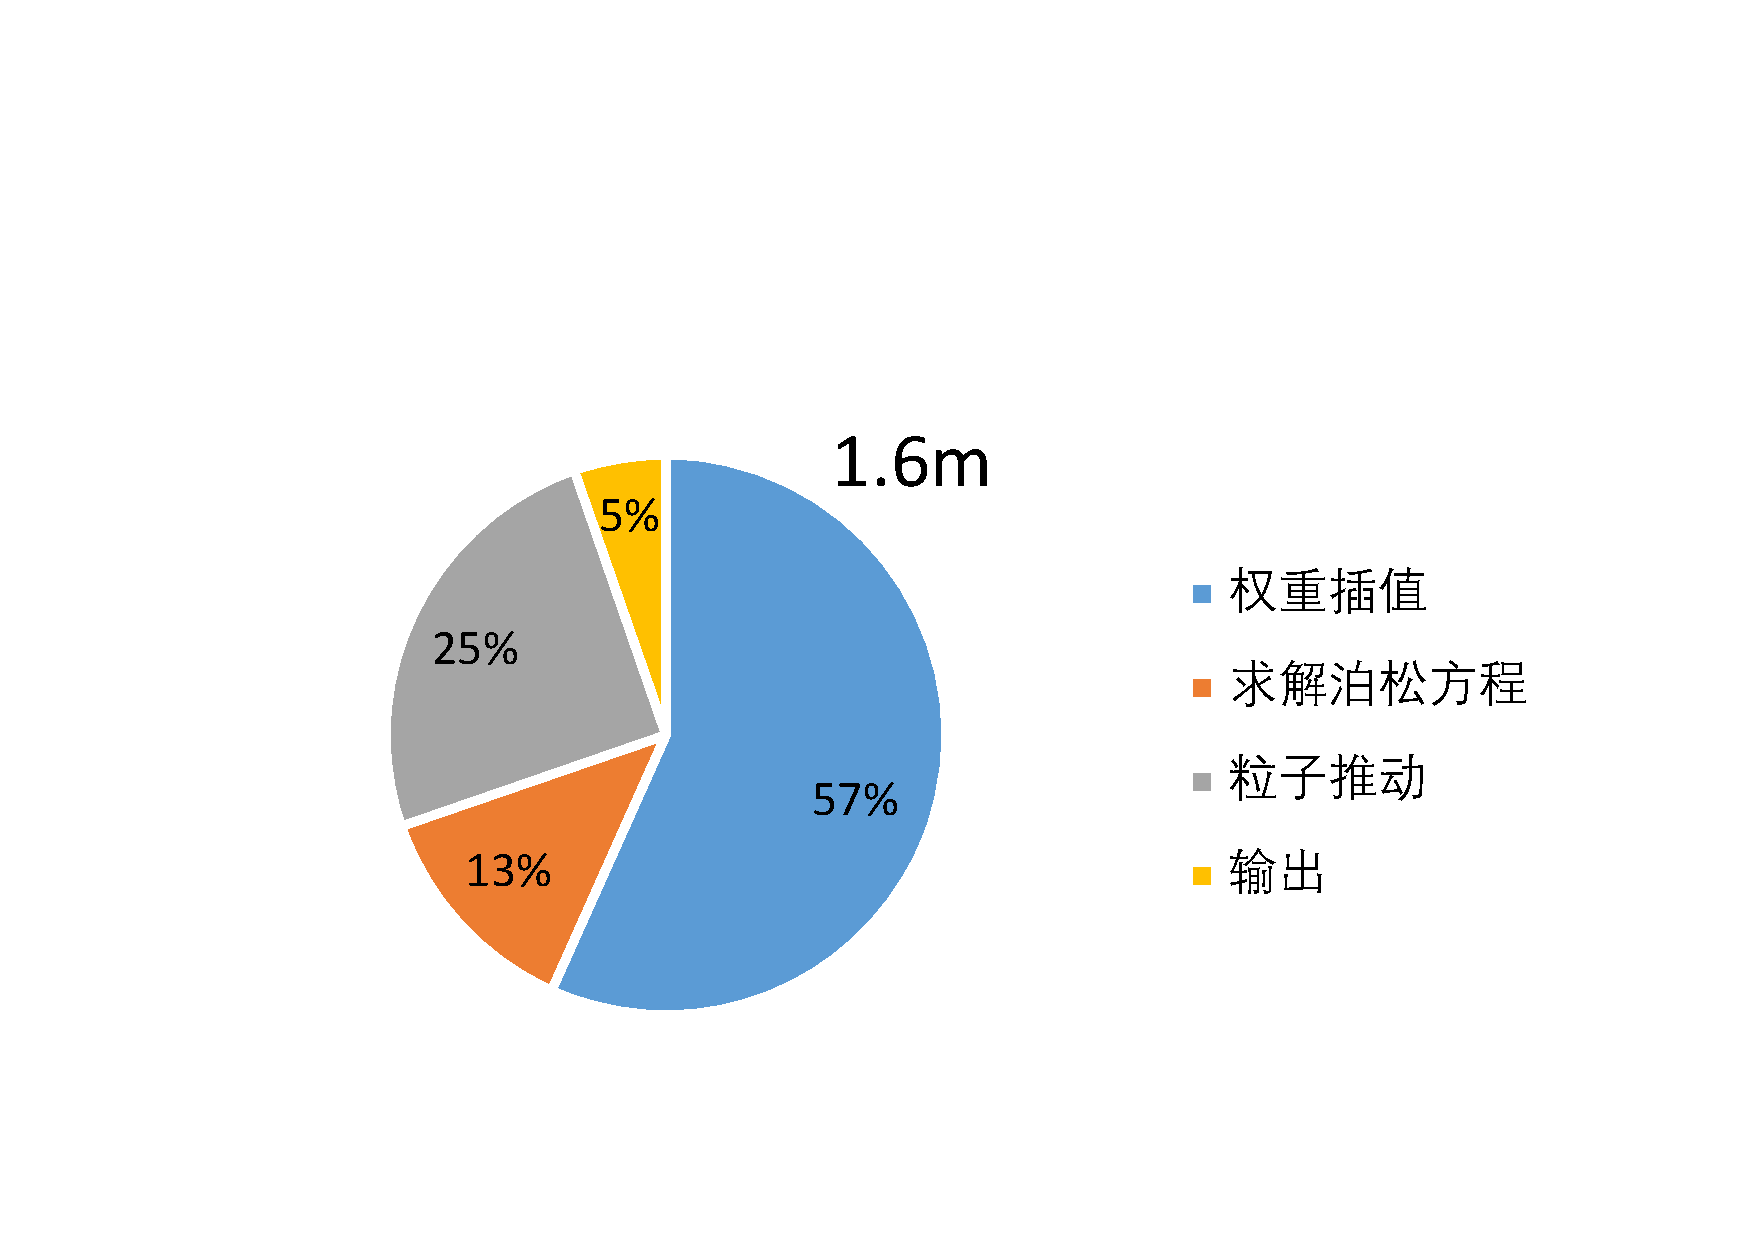
\includegraphics[width=\textwidth]{Img/PIC_speedup_1GPU_percentage3.pdf}
        %\caption{}
    \end{subfigure}
    \caption{程序各部分耗时在不同粒子数时所占百分比}\label{fig:PIC_speedup_1GPU_percentage}
\end{figure}

在上述测试中使用的都是$64 \times 64 \times 64$个格点数,因此求解泊松方程的时间和加速比都基本不变。
在不同的格点数情况下,求解泊松方程的加速比如图\ref{fig:PIC_speedup_1GPU_Poisson}所示。
可以看出,求解泊松方程的加速比随着格点数的增加逐渐变大,最终达到了接近70,这是因为格点数越大,其计算量越多,GPU上的负载能够分布得更均匀。
对于实际模拟中常用的$64 \times 64 \times 64$个格点和$128 \times 128 \times 128$个格点中,我们都取得了令人满意的加速比。

\begin{figure}[!htb]
  \centering
  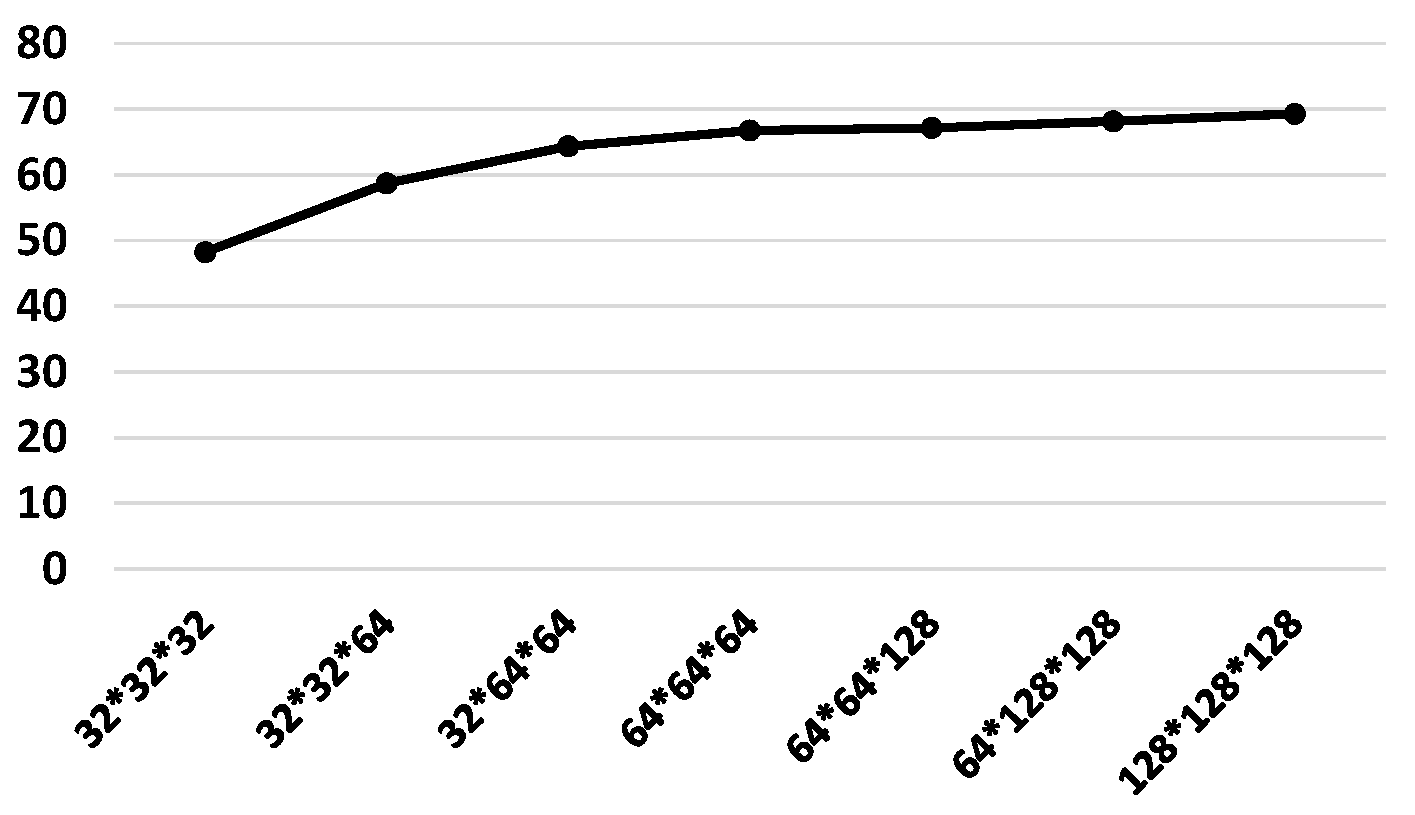
\includegraphics[width=0.9\textwidth]{Img/PIC_speedup_1GPU_Poisson.pdf}
  \caption{不同的格点数情况下单GPU求解泊松方程的加速比}
  \label{fig:PIC_speedup_1GPU_Poisson}
\end{figure}

总之,在单GPU上,程序总体的加速比达到了40,而求解泊松方程的加速比超过了60。在一个普通的家用机GPU上运行的速度相当于在64核机器上的两倍。
另外,如小节\ref{section:PIC_GPU_reorder}所述,因为GPU内存大小一般是固定的,
而不像CPU内存那样较容易的扩展,所以单GPU的粒子数目存在某个上限,当超过最大粒子数时,
应该使用多GPU来进行计算。在接下来的一节中,我们将讨论PIC程序在多GPU上的效率。

\subsection{GPU集群性能-Titan}
在单GPU测试之后,我们使用GPU集群Titan对PIC Cuda程序进行了多GPU性能测试。
Titan使用CPU和GPU混合架构,是目前世界上速度最快、规模最大的计算机集群之一。
Titan中每个节点只有一个GPU,因此只能通过使用多个节点来使用多个GPU。
在这种条件下,GPU之间的通讯只能够通过先将数据拷贝到CPU端,再通过CPU端的节点间网络进行通讯。

图\ref{fig:PIC_speedup_Titan_160k_1}为求解泊松方程时各个部分所花费的时间随GPU个数的变化。
可以看出,因为处于复制模式,求解泊松方程的耗时基本保持不变;
更多的GPU个数意味着每个GPU上的粒子数随之减小,所以粒子推动的耗时随着GPU数目的增加而减少;
而由于通讯成本随着GPU数目增加而增加,信息统计和输出耗时也随之增加。
各个部分对于GPU的数目变化的反应并不相同,单从总体来看,程序总耗时基本保持不变。

\begin{figure}[!htb]
  \centering
  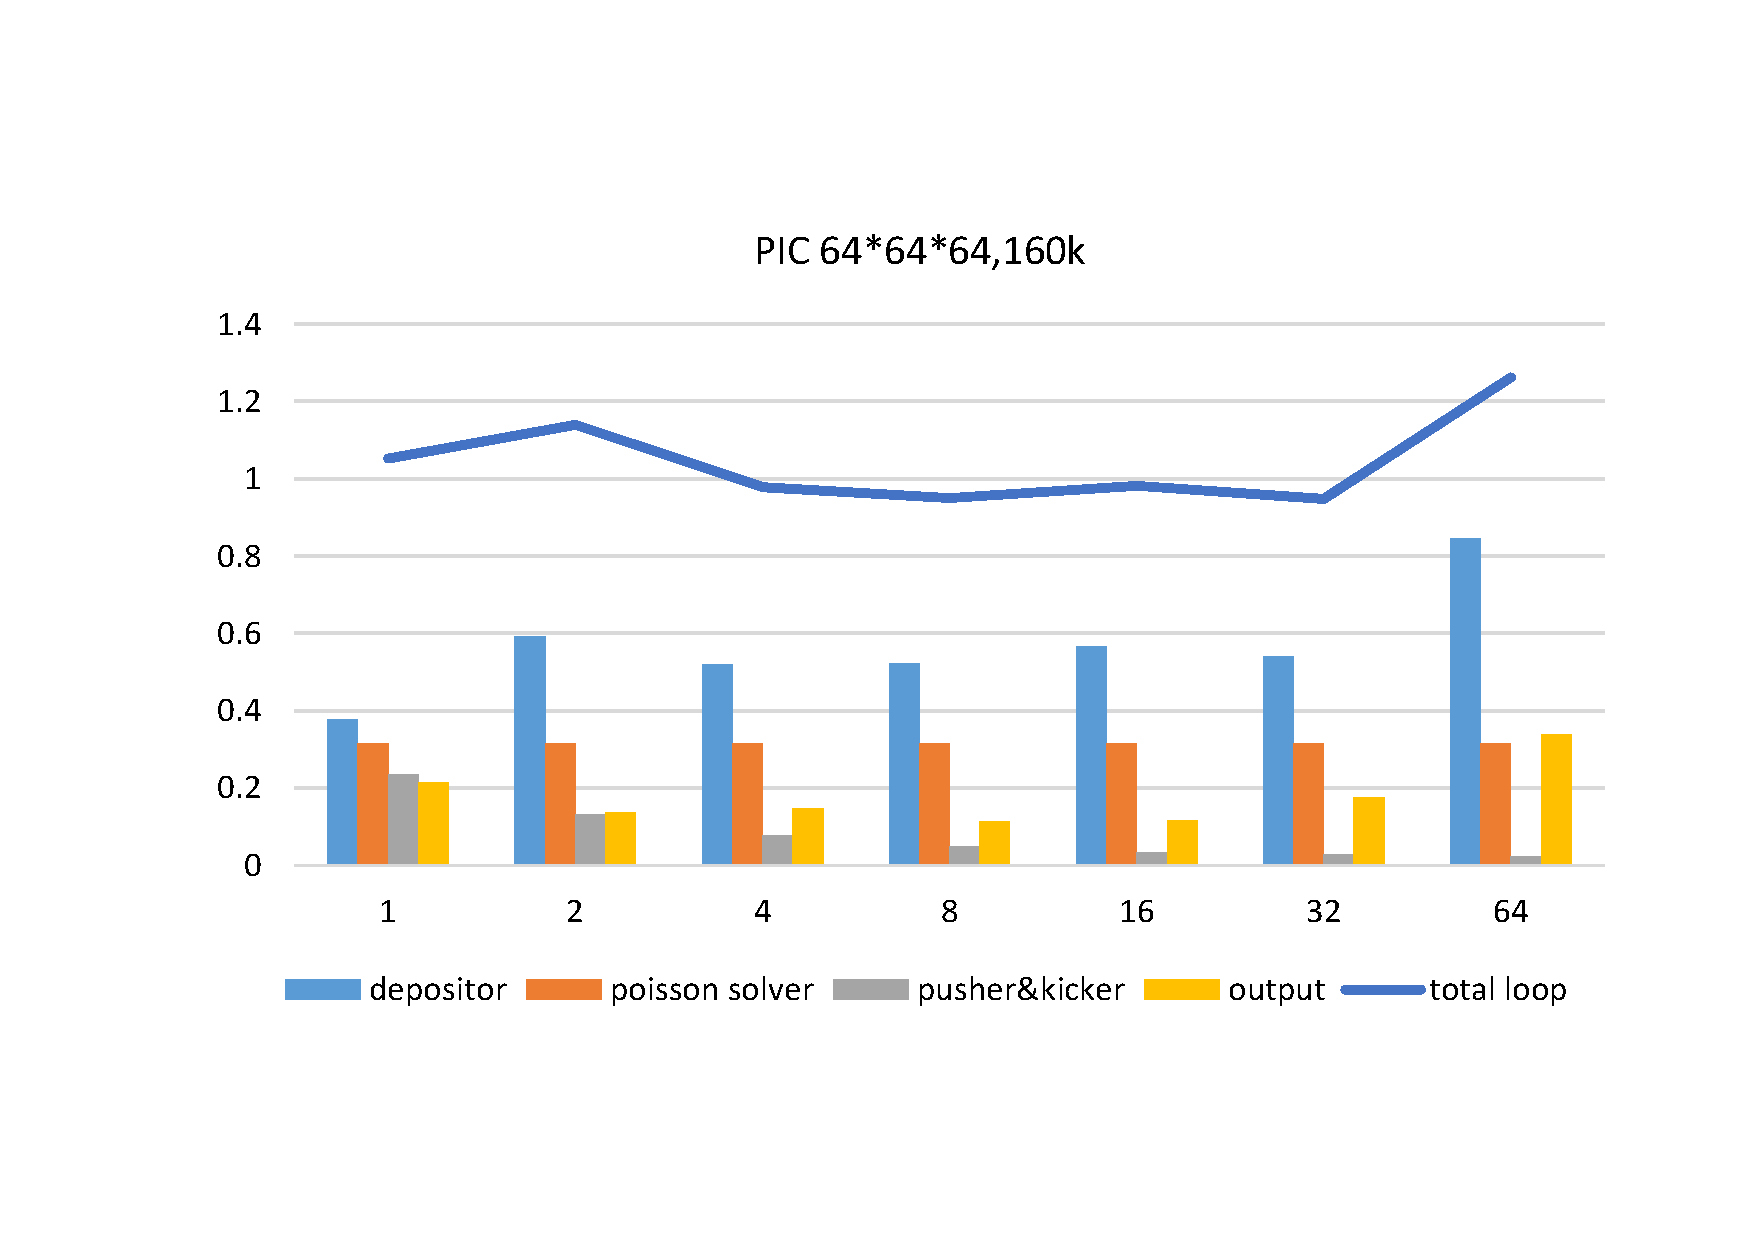
\includegraphics[width=0.9\textwidth]{Img/PIC_speedup_Titan_160k_1.pdf}
  \caption{$64 \times 64 \times 64$个格点,160K个粒子时,Titan上PIC程序耗时随GPU个数的变化}
  \label{fig:PIC_speedup_Titan_160k_1}
\end{figure}

图\ref{fig:PIC_speedup_Titan_160k_2}和图\ref{fig:PIC_speedup_Titan_160k_1}类似,也是$64 \times 64 \times 64$各个点,160k个粒子下程序总耗时随着~GPU~数目的变化。
但是在图\ref{fig:PIC_speedup_Titan_160k_2}中,GPU数目大于等于2的时候,求解泊松方程使用了域分解模式。其在各种情况下,都相较复制模式耗时更多,主要是拷贝数据花费了大量时间,这个结果和我们在小节\ref{section:PIC_GPU_Poisson}中讨论的相符。

\begin{figure}[!htb]
  \centering
  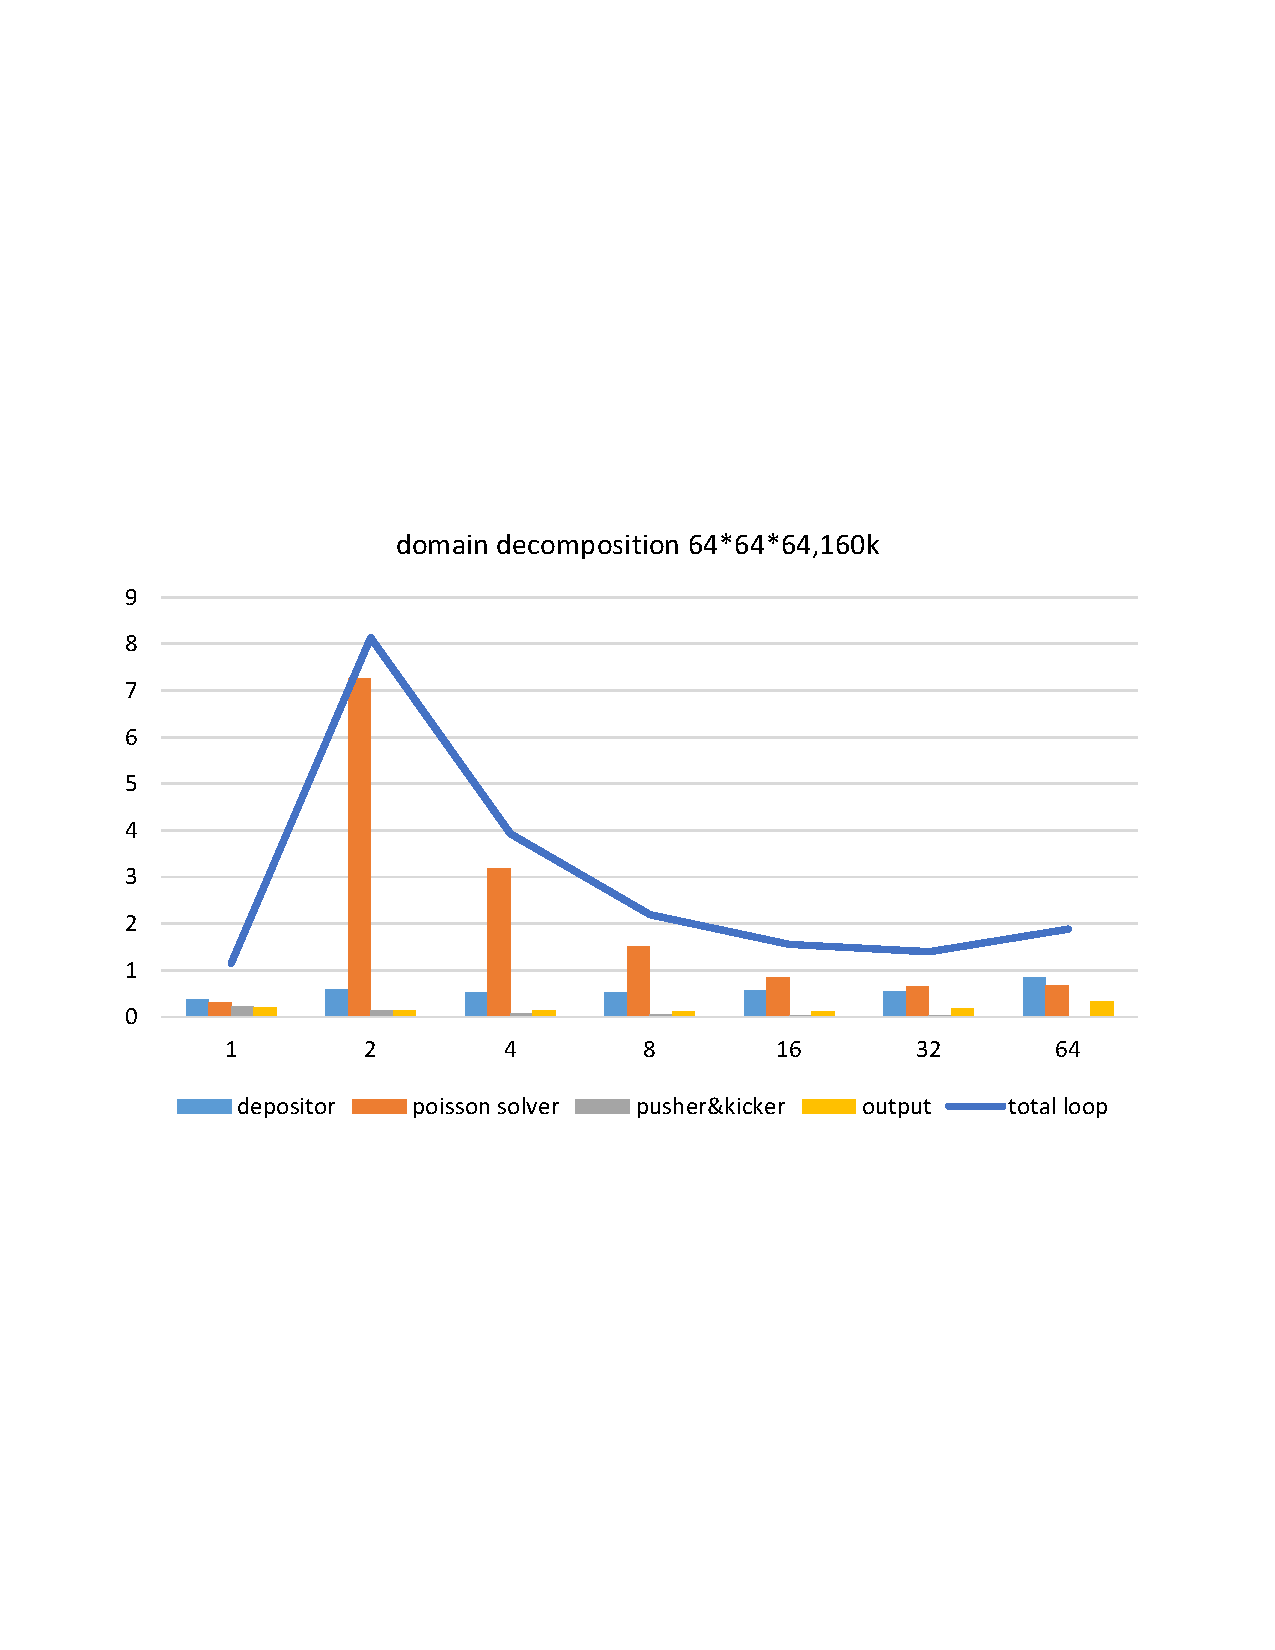
\includegraphics[width=0.9\textwidth]{Img/PIC_speedup_Titan_160k_2.pdf}
  \caption{$64 \times 64 \times 64$个格点,160Kk个粒子时,Titan上域分解模式PIC程序耗时随GPU个数的变化}
  \label{fig:PIC_speedup_Titan_160k_2}
\end{figure}

当粒子数更大时,耗时的趋势发生了变化。图\ref{fig:PIC_speedup_Titan_1_6m}是粒子数为一百六十万(~1.6m)的结果,
粒子数较图\ref{fig:PIC_speedup_Titan_160k_1}变大了十倍。在使用1.6m个粒子时,
总耗时随着使用的~GPU数目增加而明显下降,并在32个GPU处到达最小值。
这是因为在大粒子数目情况下,推动粒子和权重插值所消耗的时间占总时间的比重更大。
而由于使用多GPU带来的每个GPU上的粒子数目变少,推动粒子和权重插值能够很好的被多GPU加速。

\begin{figure}[!htb]
  \centering
  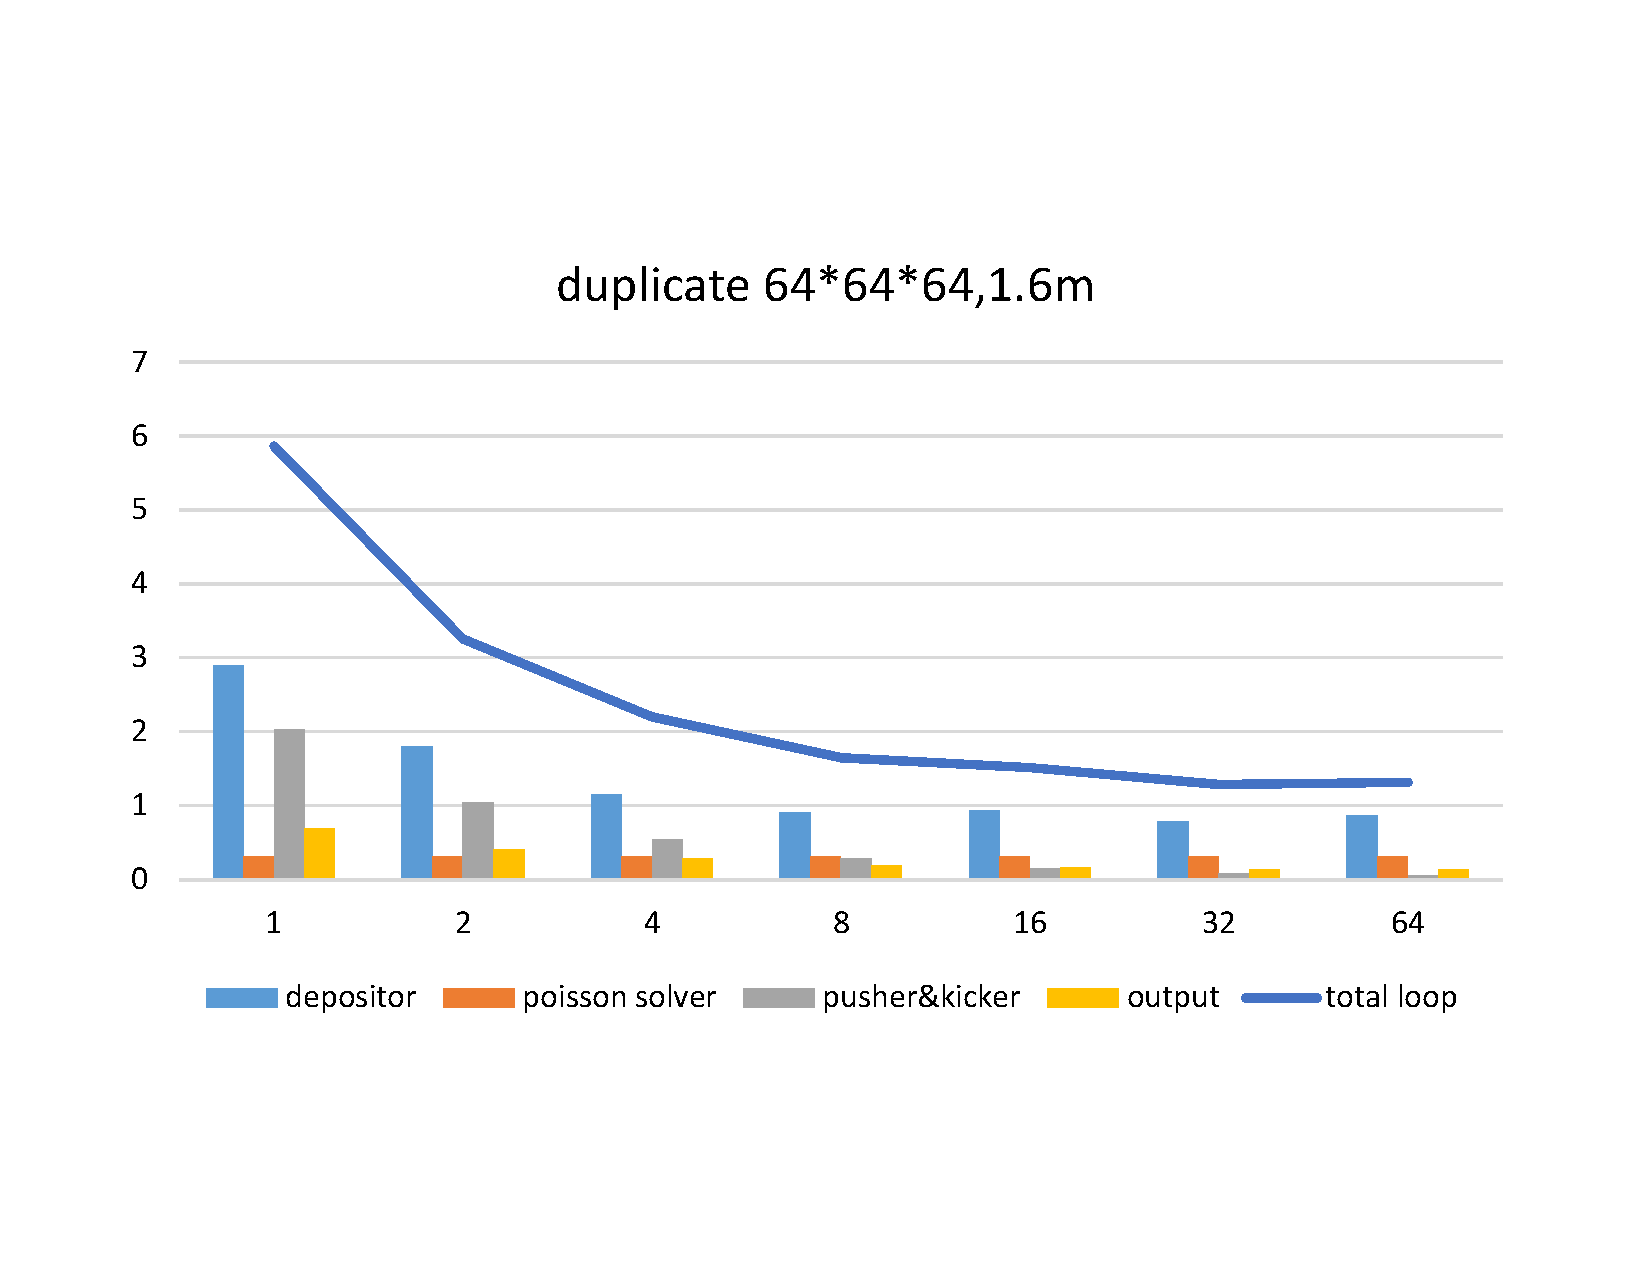
\includegraphics[width=0.9\textwidth]{Img/PIC_speedup_Titan_1_6m.pdf}
  \caption{$64 \times 64 \times 64$个格点,1.6M个粒子时,Titan上PIC程序耗时随GPU个数的变化}
  \label{fig:PIC_speedup_Titan_1_6m}
\end{figure}

我们尝试了使用更大的粒子数,一千六百万个粒子(16m),更十倍于前,如图\ref{fig:PIC_speedup_Titan_16m}所示。
由于GPU内存大小的限制,程序在这个粒子数下不能仅仅使用1或2个~GPU运行,因此在图\ref{fig:PIC_speedup_Titan_16m}中,
GPU数目等于1和等于2的时候没有数据。对于更多的GPU数目,程序耗时随着GPU数目增加而减小。

超级计算机Titan上使用的GPU型号为NVIDIA K20x,每个GPU有5GB的内存。
理想情况下,一个5GB内存能够使用的最大粒子数为六千万(60m)。
但这个粒子数是在使用空间均匀分布下才能达到,而实际上,我们很难达到这个粒子数。
在一个实际的加速器模拟中,我们通常使用WaterBag 或者高斯分布,因此其可用的粒子数目远小于理想数目。

\begin{figure}[!htb]
  \centering
  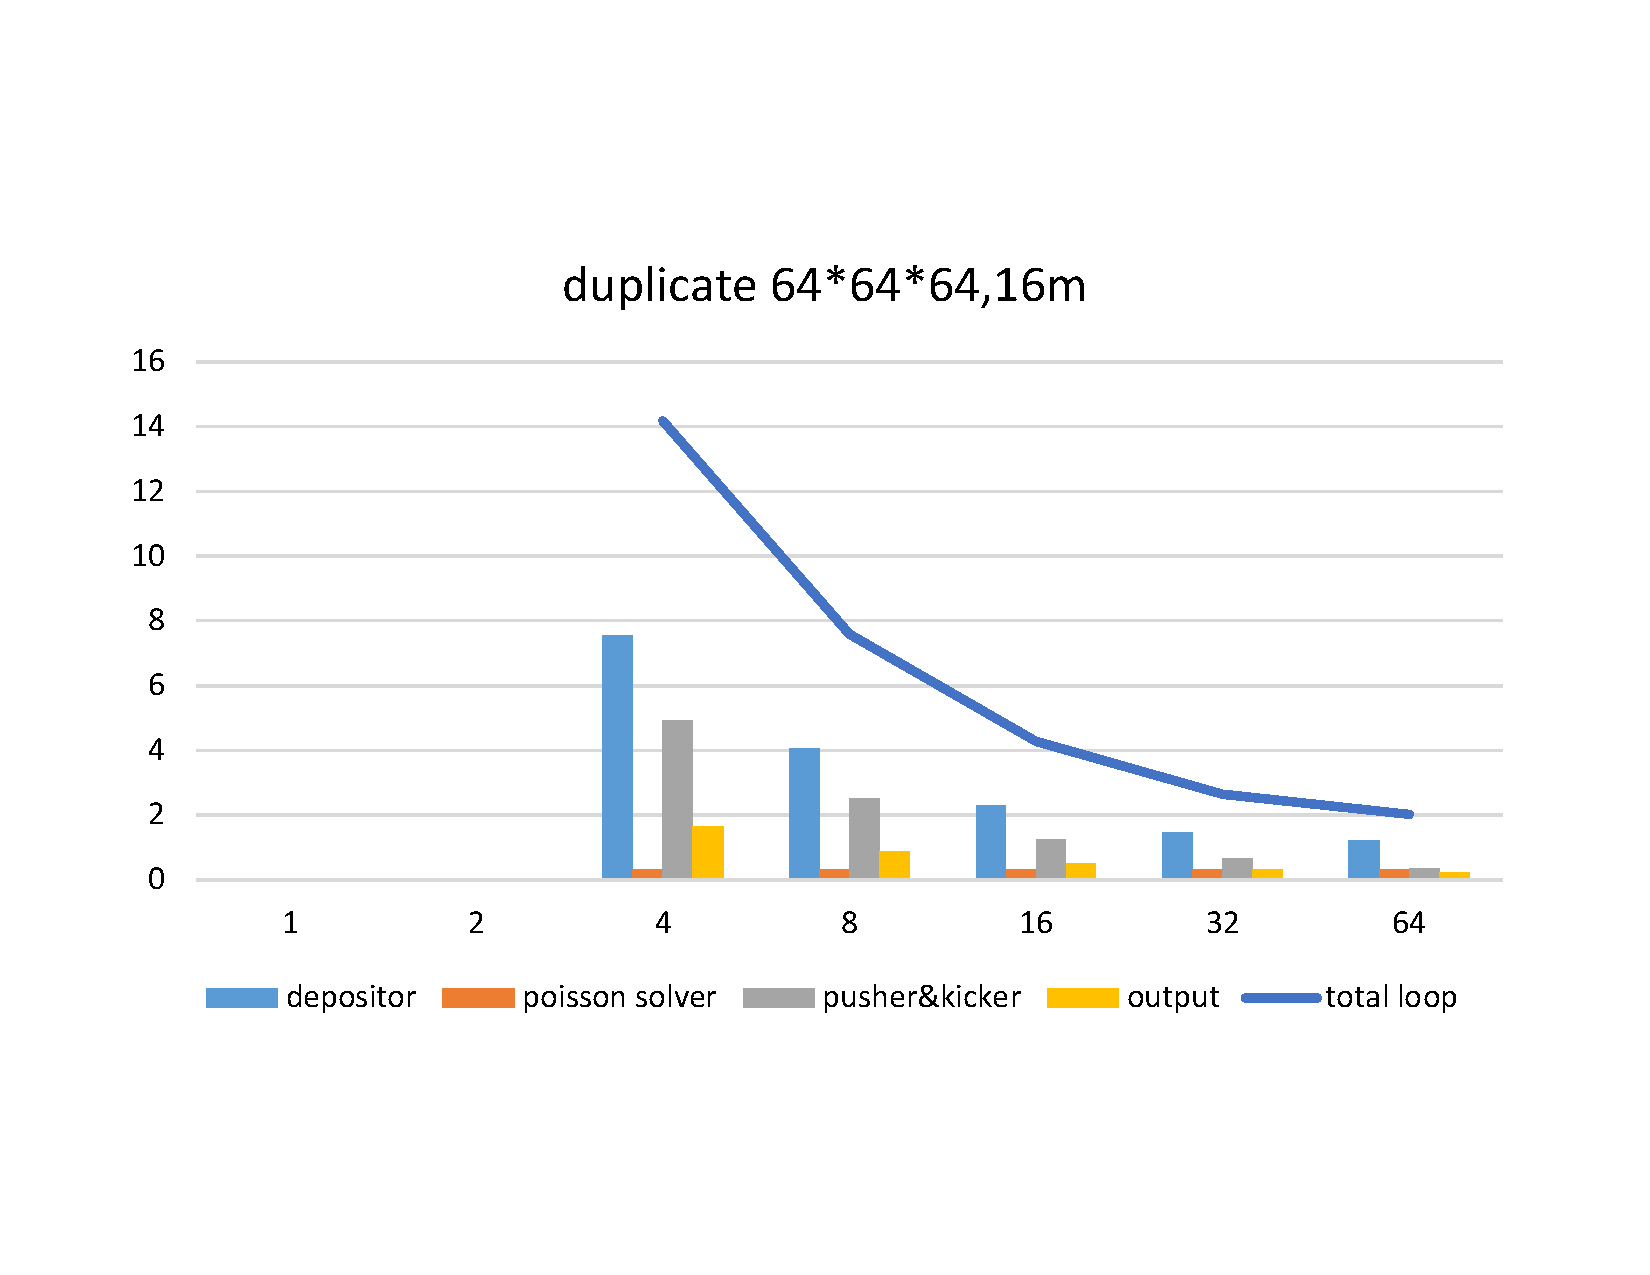
\includegraphics[width=0.9\textwidth]{Img/PIC_speedup_Titan_16m.pdf}
  \caption{$64 \times 64 \times 64$个格点,16M个粒子时,Titan上PIC程序耗时随GPU个数的变化}
  \label{fig:PIC_speedup_Titan_16m}
\end{figure}

\subsection{GPU集群性能-SummitDev}
和上一节中在Titan上进行的性能研究类似,我们还在ORNL新一代的GPU集群SummitDev上对PIC-Cuda程序进行了测试。
图~\ref{fig:PIC_SummitDev_160K}为使用 $64\times64\times64$ 个格点和  160K 个粒子的程序耗时。
和Titan的耗时趋势一样,随着GPU数量的增加,粒子推动所消耗的时间减少,权重粒子所消耗的时间有所增加。
而总时间并不随着GPU数量的增加而减少。多GPU不能提高效率的原因是SummitDev上GPU的计算能力非常强大,
对于160K个粒子来说,纯计算在整体耗时中所占比例不大,使用一个GPU已经足够。

\begin{figure}[!htb]
  \centering
  \includegraphics[width=0.9\linewidth]{Img/PIC_SummitDev_160K.pdf}
  \caption{$64 \times 64 \times 64$个格点,160K个粒子时,SummitDev上PIC程序耗时随GPU~个数的变化}
  \label{fig:PIC_SummitDev_160K}
\end{figure}

当粒子数量变大时,耗时趋势发生了变化。
图~\ref{fig:PIC_SummitDev_1600K}显示了160万个粒子的结果。总耗时随着GPU数量的增加而减少,并在16个GPU时到达最小值。
与Titan上的运行时间相比,由于计算能力的提高,对于同一规模的问题在SummitDev上所需要的时间减少了50\% 。
图~\ref{fig:PIC_SummitDev_16M}为了1600万个粒子的结果,受GPU内存大小的限制,程序必须使用两个或两个以上GPU运行。
在粒子数很大的情况下,由于计算量较大,程序能够充分使用多个GPU的性能,所以总耗时随着GPU数目的增加而单调递减。

\begin{figure}[!htb]
  \centering
  \includegraphics[width=0.9\linewidth]{Img/PIC_SummitDev_1600K.pdf}
  \caption{$64 \times 64 \times 64$个格点,1.6M个粒子时,SummitDev上PIC程序耗时随GPU~个数的变化}
  \label{fig:PIC_SummitDev_1600K}
\end{figure}

\begin{figure}[!htb]
  \centering
  \includegraphics[width=0.9\linewidth]{Img/PIC_SummitDev_16M.pdf}
  \caption{$64 \times 64 \times 64$个格点,16M个粒子时,SummitDev上PIC程序耗时随GPU~个数的变化}
  \label{fig:PIC_SummitDev_16M}
\end{figure}

\subsection{CPU集群性能-KNL}        \label{section:PIC_Performance_CPUcluster}
为了和GPU做比较,我们也在CPU集群KNL上使用MPI~和OpenMP混合并行实现了高效率的PIC程序。
首先,我们使用集群的一个节点来研究不同 OpenMP 线程数和MPI进程数下程序的效率和内存占用情况,并找到最优混合并行配置。
之后,我们使用多个节点,研究程序在不同节点数下的效率变化。

\subsubsection{单节点}
首先,我们使用$64 \times 64 \times 64$个网格,在1.6m粒子数下测试不同的混合并行配置,
如图\ref{fig:PIC_speedup_Cori_1node_1_6m}所示。其中横轴为不同的并行配置,
其中MPI进程数由1指数增加到64,而~OpenMP~线程数有64指数得减小到1,线程数乘以进程数则保持不变。
在每种并行配置下,总时间(浅蓝色实线),和权重插值,求解泊松方程,推动粒子,
信息输出(各色柱行)所耗时间由左纵轴以秒为单位表示,而内存占用(绿色实线)由右纵轴以GB为单位表示。

\begin{figure}[!htb]
  \centering
  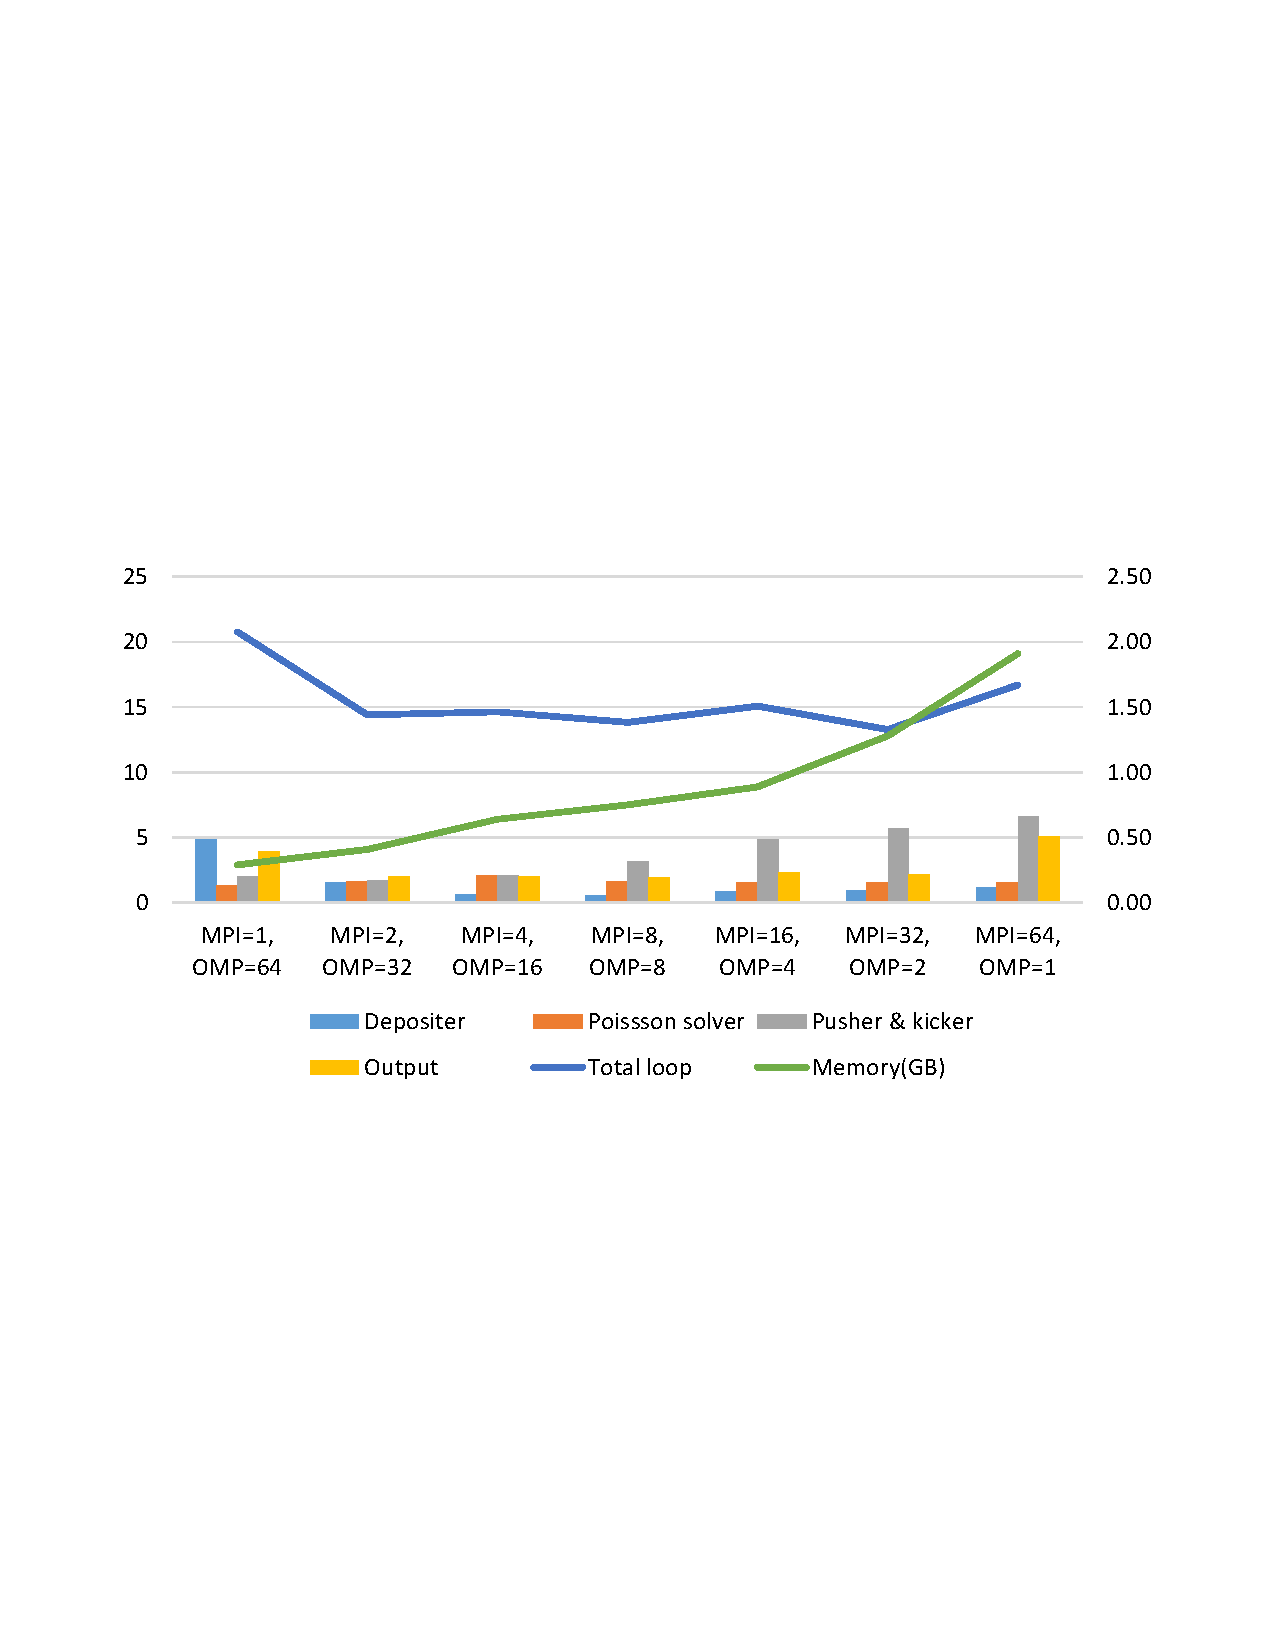
\includegraphics[width=0.9\textwidth]{Img/PIC_speedup_Cori_1node_1_6m.pdf}
  \caption{1.6m粒子数下,单节点下不同混合并行配置的耗时与内存占用}
  \label{fig:PIC_speedup_Cori_1node_1_6m}
\end{figure}

从图\ref{fig:PIC_speedup_Cori_1node_1_6m}可以看出,除了纯OpenMP并行(MPI=1,OMP=64)明显较慢外,
其他各个并行配置下所消耗的总时间的差别并不大,其中耗时最小的并行配置为使用32个MPI进程,每个进程使用2个OpenMP线程。
%一般而言,使用较大的MPI进程数是比较有效率的选择。
而内存占用基本随着MPI进程数目线性增加。

程序的不同部分对于并行配置的反应并不相同。随着MPI进程数的增加和每个进程所用线程数的减小,权重插值的耗时先减小后增加,一开始先从MPI=64,OMP=1时的1.14秒减少到了MPI = 8,OMP =8时的0.58秒,然后其开始剧烈增加,最终到达MPI = 1,OMP =64时的4.85秒。其原因是权重插值需要在不同的线程之间进行归约以避免线程冲突,而归约操作在线程数很大时有一个较大的启动时间。粒子推动耗时随着MPI数变大单调增加,这是因为OpenMP更适合KNL众核架构,并能更有效的利用矢量处理器。

我们也测试了不同的粒子数下的并行配置,测试的粒子数为160k和16m,分别是之前粒子数的十分之一和十倍,其结果如图\ref{fig:PIC_speedup_Cori_1node_160k}和图\ref{fig:PIC_speedup_Cori_1node_16m}所示。
在160k个粒子的情况下,总时间随着MPI进程数的增加单调减少,这表明小粒子数情况更适合纯MPI并行。
而在1.6m个粒子的情况下,纯OpenMP并行由于无MPI进程间通讯,显示出一些优势,但是其总耗时依然大于MPI并行,其耗时最小的配置为MPI=64,OMP=1。
在两种情况下,内存占用总是随着MPI进程数变大而单调增加。

\begin{figure}[!htb]
  \centering
  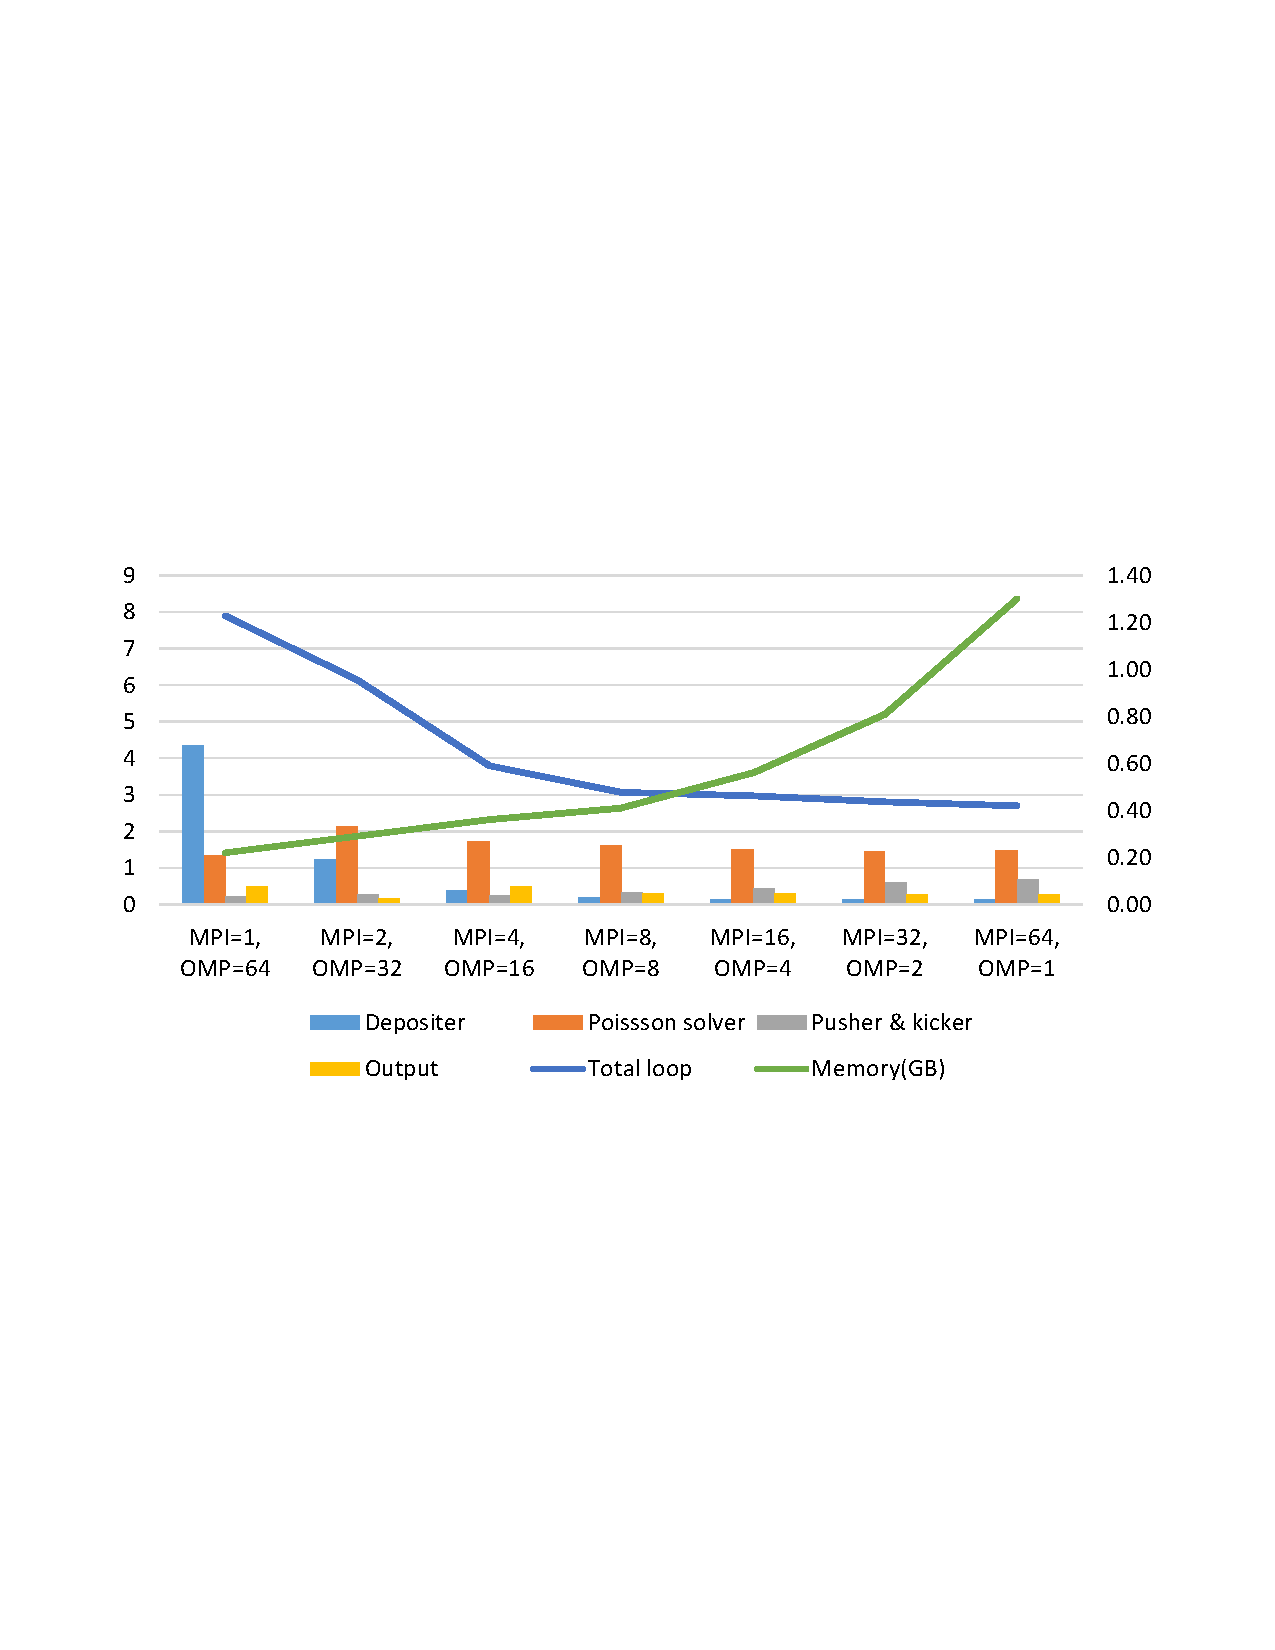
\includegraphics[width=0.9\textwidth]{Img/PIC_speedup_Cori_1node_160k.pdf}
  \caption{160k粒子数下,单节点下不同混合并行配置的耗时与内存占用}
  \label{fig:PIC_speedup_Cori_1node_160k}
\end{figure}

\begin{figure}[!htb]
  \centering
  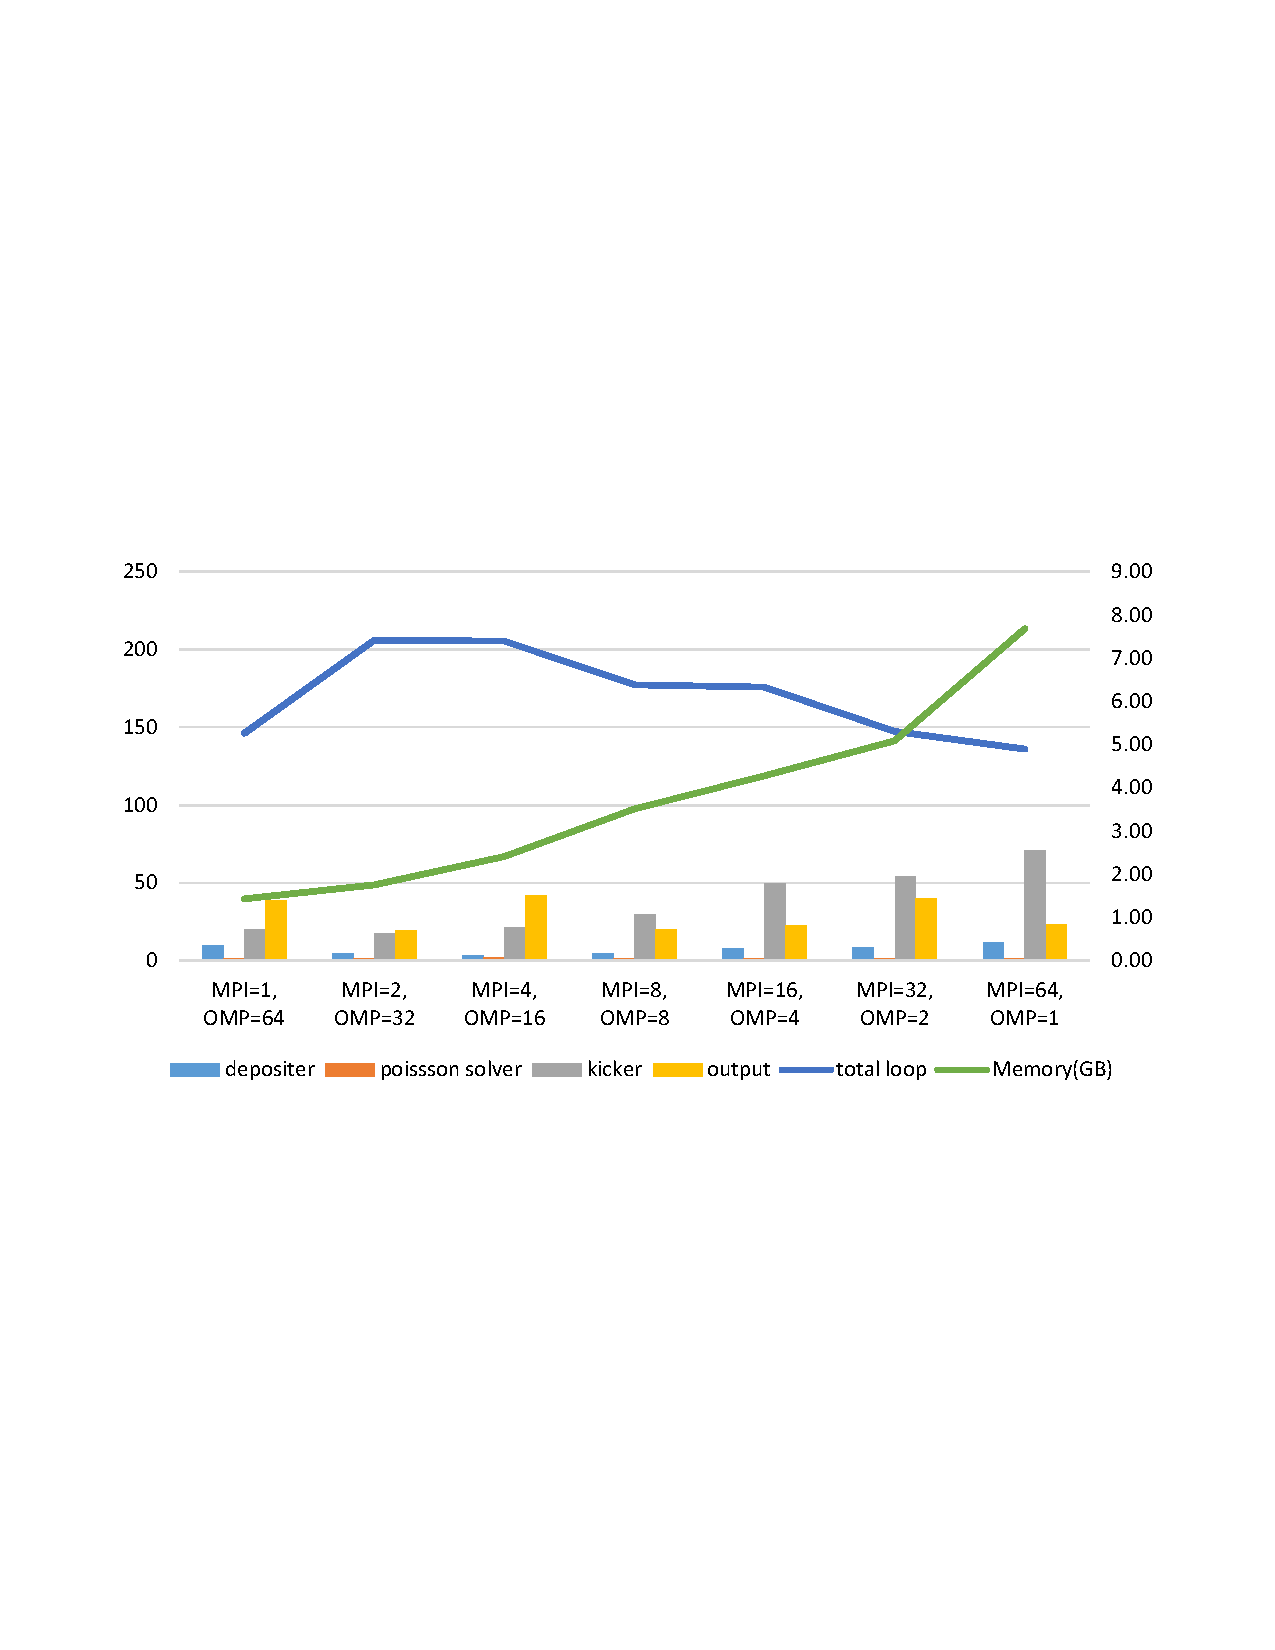
\includegraphics[width=0.9\textwidth]{Img/PIC_speedup_Cori_1node_16m.pdf}
  \caption{16m粒子数下,单节点下不同混合并行配置的耗时与内存占用}
  \label{fig:PIC_speedup_Cori_1node_16m}
\end{figure}


\subsubsection{多节点}
从上面单节点的测试中可以得到,使用较大的MPI进程数和较小的OpenMP 线程数是更有效率的并行配置。
因此在多节点的测试中,我们首先选用纯MPI并行,测试在不同的节点数下程序总体以及各个部分的耗时情况。之后,我们也测试了OMP=2和OMP=4的情况,并与纯MPI程序进行了比较。

图\ref{fig:PIC_speedup_Cori_scalability}是纯MPI配置下PIC程序在CPU集群多节点下的耗时情况。
图中横轴为节点数目,每个节点使用64个核;左纵轴为时间,以秒为单位;
右纵轴为内存使用,以GB为单位。随着使用更多的节点,程序总耗时先降低后增加,
在32个节点处到达最小值。总耗时先减小是因为使用的节点数越多,每个节点上需要进行的运算越少;
后增加是因为随着节点数上升,节点间的通讯时间也会随之增加。
图\ref{fig:PIC_speedup_Cori_percetage_64nodes}为使用64个节点时程序各个部分消耗时间所占的百分比,
可以看出此时通讯耗时已经占了总耗时的60\%。

\begin{figure}[!htb]
  \centering
  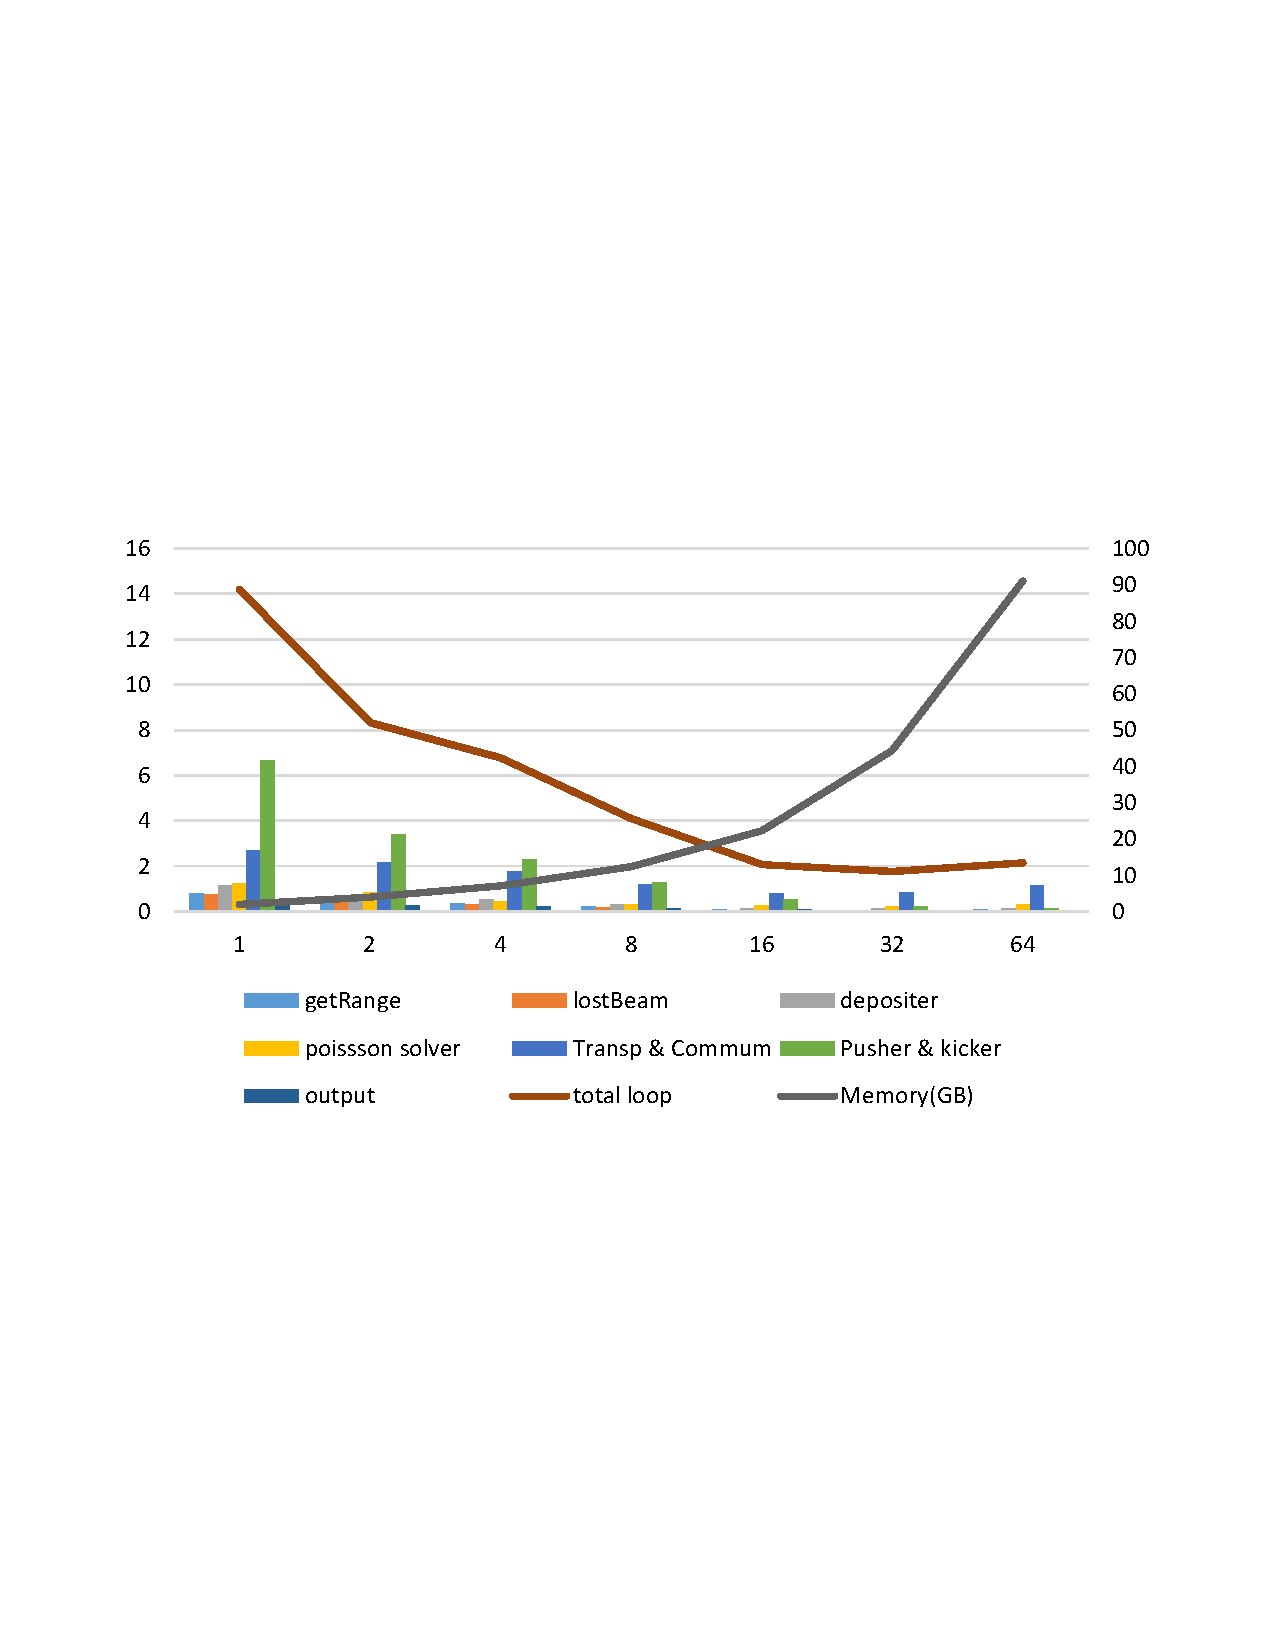
\includegraphics[width=0.9\textwidth]{Img/PIC_speedup_Cori_scalability.pdf}
  \caption{PIC程序使用多个CPU节点的耗时}
  \label{fig:PIC_speedup_Cori_scalability}
\end{figure}

\begin{figure}[!htb]
  \centering
  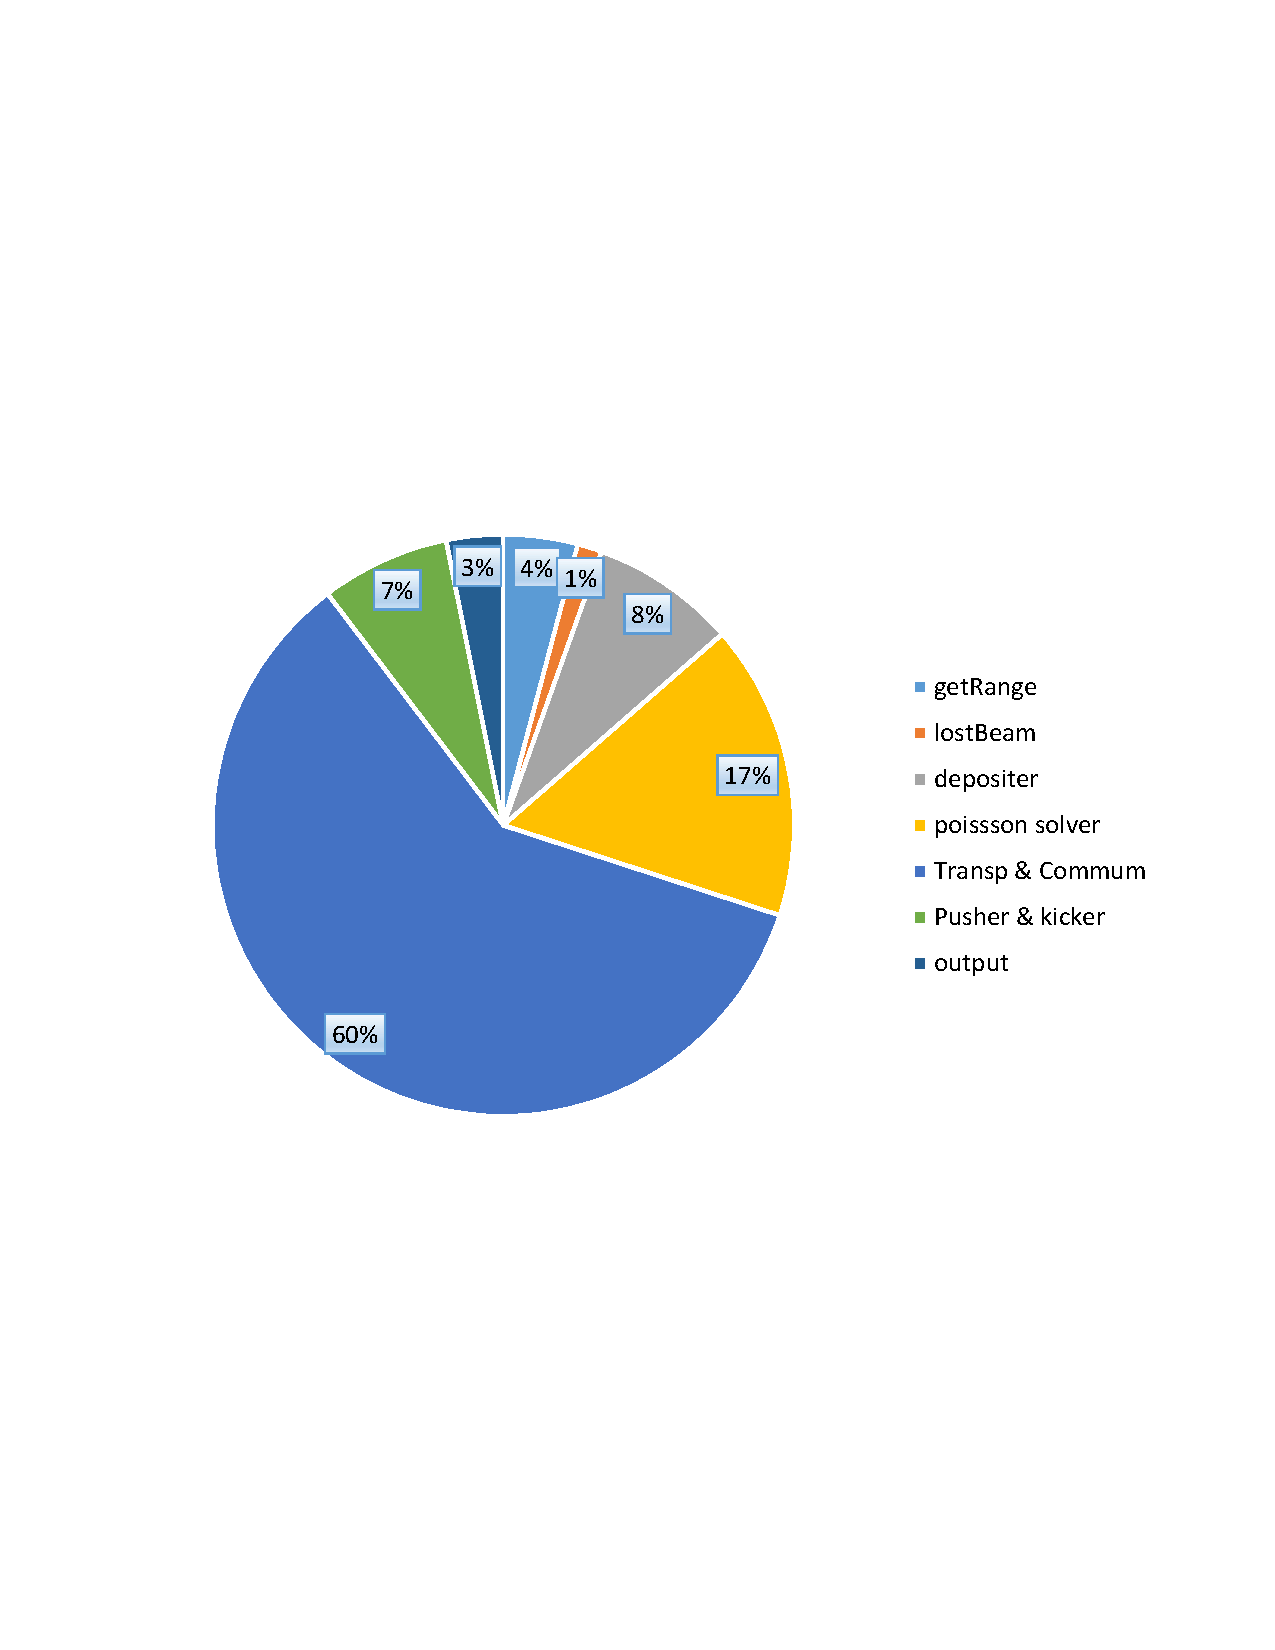
\includegraphics[width=0.5\textwidth]{Img/PIC_speedup_Cori_percetage_64nodes.pdf}
  \caption{使用64个节点时程序各个部分消耗时间所占的百分比}
  \label{fig:PIC_speedup_Cori_percetage_64nodes}
\end{figure}

接下来,我们对OMP=2和OMP=4进行了测试,并与纯MPI程序(OMP=1)进行了比较,如图\ref{fig:PIC_speedup_Cori_multi_nodes_timeMemory}所示。
在大部分情况下,不同并行配置的耗时差别很小;但是在某些情况下差别很大,比如节点数为16时,纯MPI的速度是OMP=4的 1.8倍。
对于内存使用情况, 使用更多的OpenMP线程和更少的MPI进程总是占优势。
综合考虑,在内存足够大的情况下,使用纯MPI并行配置在KNL上运行PIC程序依然是一个很好的选择。

\begin{figure}[!htb]
    \centering
    \begin{subfigure}[b]{0.48\textwidth}
        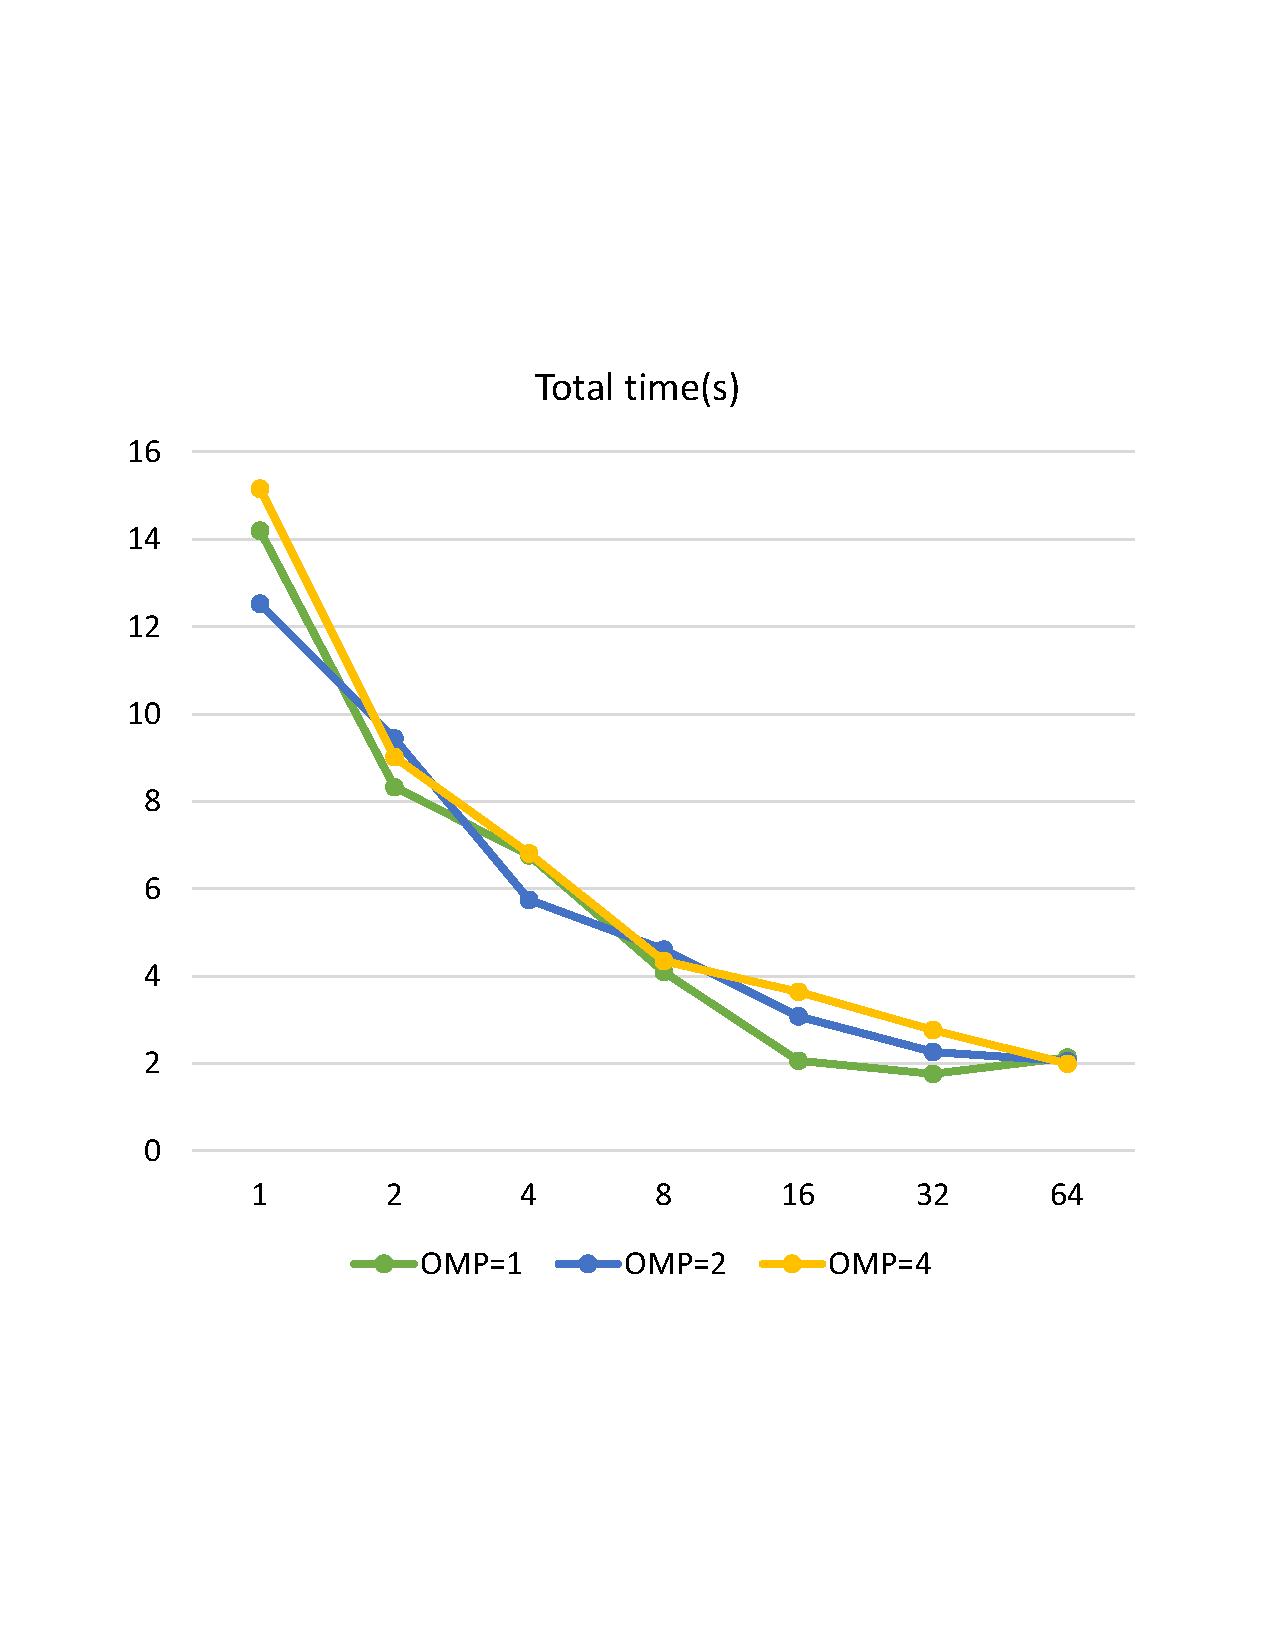
\includegraphics[width=\textwidth]{Img/PIC_speedup_Cori_multi_nodes_time.pdf}
        \caption{耗时}
    \end{subfigure}
    \begin{subfigure}[b]{0.48\textwidth}
        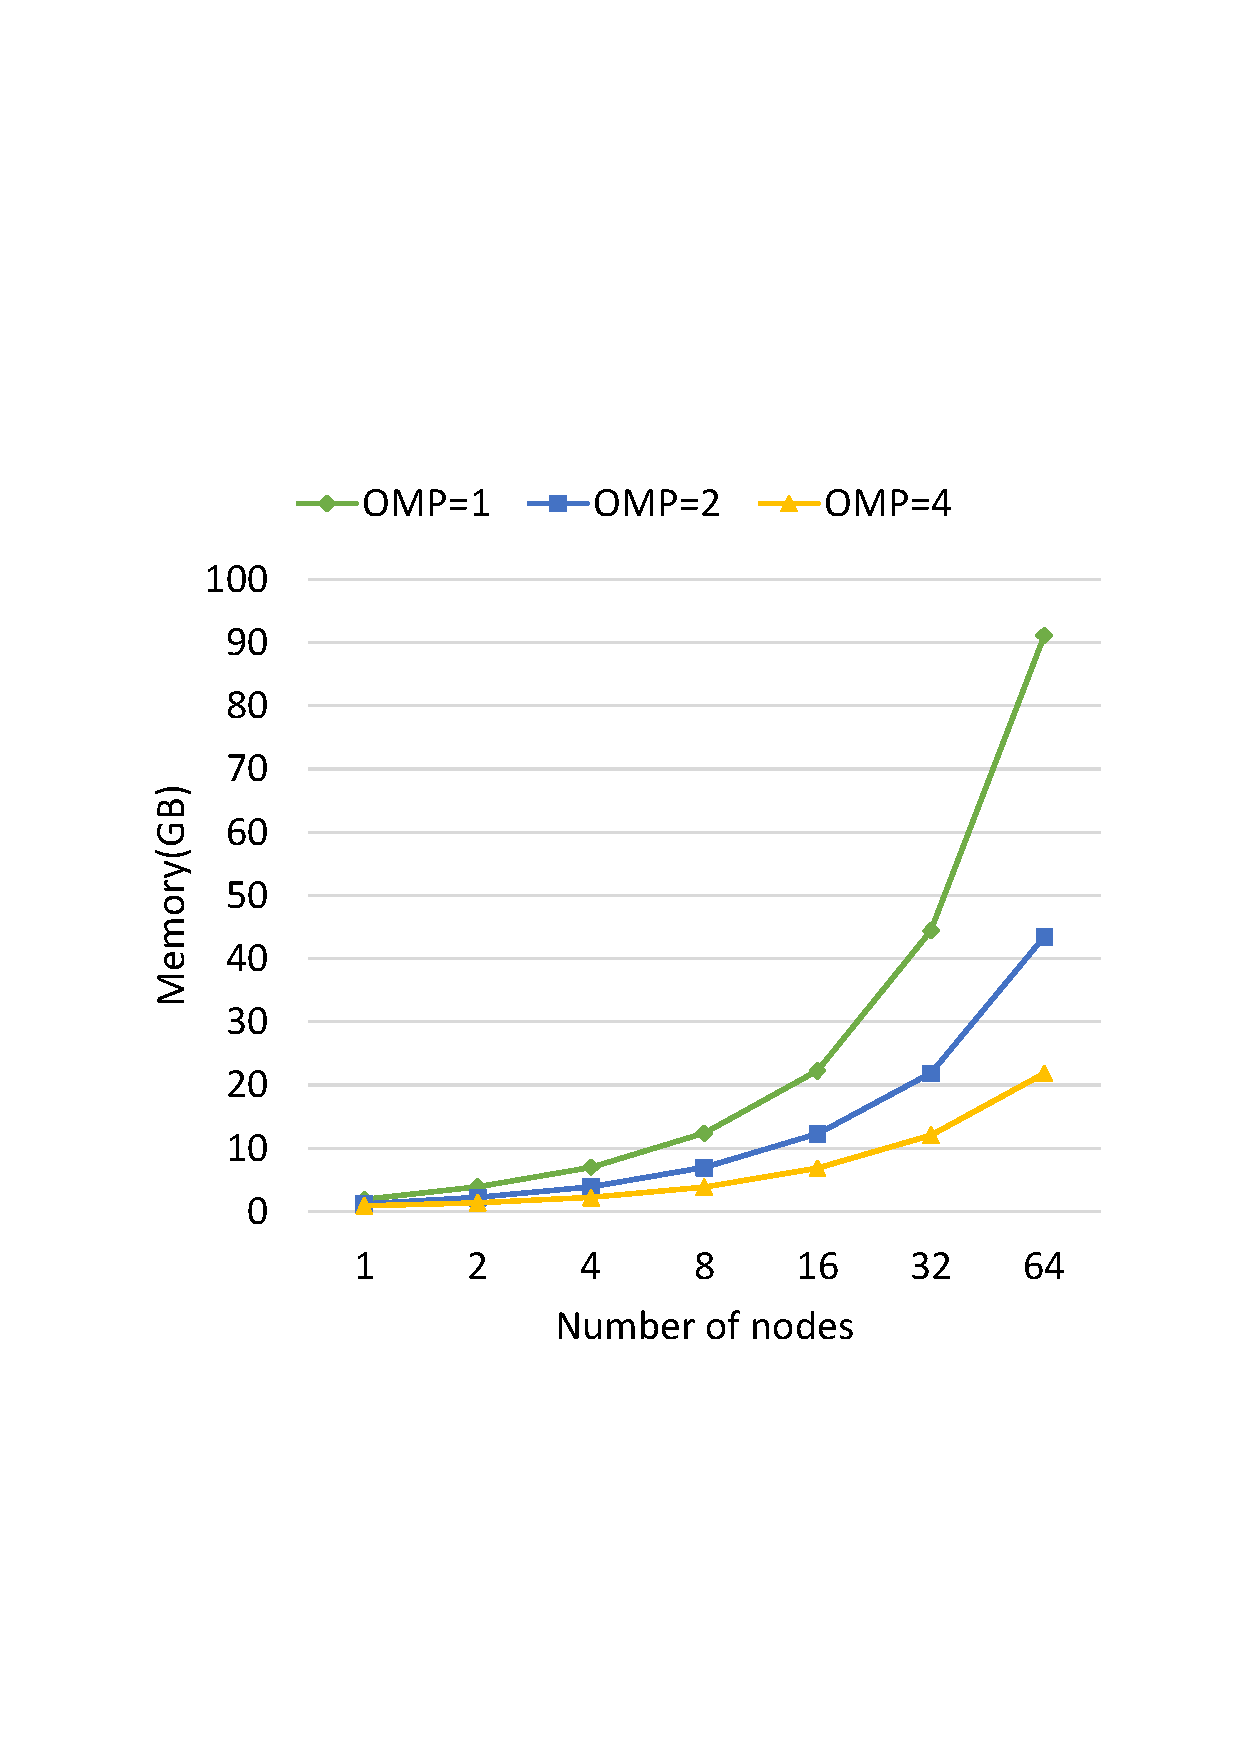
\includegraphics[width=\textwidth]{Img/PIC_speedup_Cori_multi_nodes_memory.pdf}
        \caption{内存占用}
    \end{subfigure}
    \caption{不同并行配置下的多节点运行情况比较}
    \label{fig:PIC_speedup_Cori_multi_nodes_timeMemory}
\end{figure}

\subsubsection{与GPU对比}

在之前第\ref{section:PIC_Performance_GTX1060}节的单GPU测试中,我们使用的GPU型号为GTX 1060,
其包含1280颗核心,时钟频率为1.71GHz。而在本节我们使用的CPU型号为Intel® Xeon Phi™ Processor 7250 (KNL),
共包含68颗核心,时钟频率为1.40GHz,但是实际上为了方便比较,我们只是使用了64颗核心。

而由于GPU程序做了一些简化,缺少一部分步骤,例如粒子丢失判据等,我们在进行比较的时候也在CPU程序的耗时中减去了相应部分。
在$64 \times 64 \times 64$个格点数,1.6m个粒子的情况下,对于同样长度的加速器,使用一个GPU代码的总耗时为3.56秒,
这类似于CPU程序在300个核心上的运行时间。换而言之,对于我们实现的PIC程序,一个GPU卡的运算效率与4到8个CPU节点的运行效率相当。


\section{Symplectic算法性能}        \label{section:Symplectic_performance}
使用一个GPU,Symplectic算法与CPU串行相比实现了超过400倍的加速。
而且,加速比会随着GPU的数目几乎线性增长。我们对GPU程序的性能和可拓展性进行了两个测试,
第一个测试使用一个普通的家用GPU:GTX 1060 6GB,测试的结果与在CPU串行运行的程序进行比较。
第二个测试使用ORNL的GPU集群Titan,用于测试程序的可扩展性,即程序在多GPU下的表现。

\subsection{单GPU性能提升-GTX1060}
首先,我们将GPU代码的性能与CPU代码进行比较。GPU代码使用GeForce GTX 1060 6GB(Pascal架构)进行测试,而作为对比的CPU代码使用AMD Opteron 6134的一个核心运行,测试的软件环境为Ubuntu 16.04,使用CUDA 8.0版。

加速比由CPU版本运行的运行时间除以GPU版本的运行时间得到。在本次测试中,我们对空间电荷求解器和整个程序分别进行了比较。
空间电荷求解器包括将数据从CPU侧复制到GPU侧,计算空间电荷效应,推动粒子,并将数据复制回CPU侧,
而整个程序则包括了除了空间电荷求解器之外的所有其他部分,比如外场推动,输入,统计,输出等等。

从CPU代码简单的移植到GPU上就可以实现大约200倍的加速,并且通过优化可以获得更大的加速比。
在采用了小节\ref{section:symplectic_GPU}中的优化策略后,程序能够充分利用GPU,取得了超过400的加速比。
接下来,如图\ref{fig:OneGPU}所示,我们会讨论分别讨论空间电荷效应和整个程序在不同的问题规模大小下的加速比。

\begin{figure}[!htb]
    \centering
    \begin{subfigure}[b]{0.9\textwidth}
        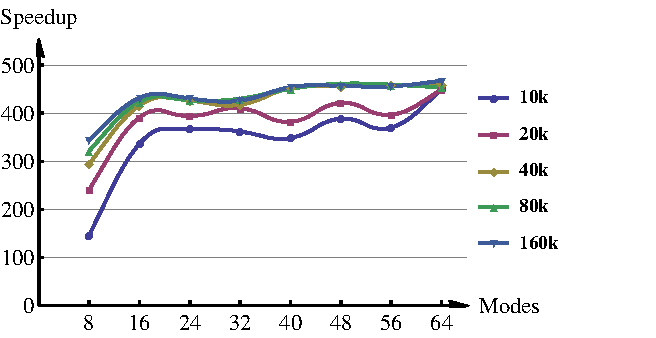
\includegraphics[width=\textwidth]{SymplecticSpaceChargeGPU_AMD13th.pdf}
        \caption{空间电荷效应求解器加速比}
        \label{fig:SCOpt}
    \end{subfigure}
    \quad
    ~ %add desired spacing between images, e. g. ~, \quad, \qquad, \hfill etc.
      %(or a blank line to force the subfigure onto a new line)
    \begin{subfigure}[b]{0.9\textwidth}
        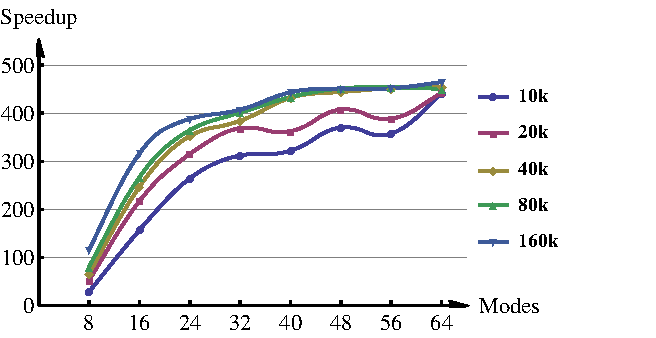
\includegraphics[width=\textwidth]{SymplecticTotalGPU_AMD13th.pdf}
        \caption{程序整体加速比}
        \label{fig:TotalOpt}
    \end{subfigure}
    \caption{单GPU加速比}\label{fig:OneGPU}
\end{figure}

图\ref{fig:SCOpt}为优化后的空间电荷效应求解器的加速比在不同的问题规模下的变化。
其中,横坐标为展开的阶数,而纵坐标是加速比,不同的曲线是不同粒子数目的结果。
可以看到,阶数越大加速比越高,这与我们的预期符合,因为阶数越大意味着空间电荷求解器占用的时间在总时间中的比例越大。
其中,在$8\times8\times8$阶时加速比很低是因为在这种模式下的计算量很低。
随着阶数的增加程序计算量也随之增加,GPU的负载更为平衡,因此取得了更大的加速比。
另一方面,粒子数目对于加速比的影响很小,在大阶数的情况下尤为如此。
这是因为粒子数目本身远远超出了一个GPU的核心数目(在GTX 1060 上为1280个核心),
即使在最低粒子数(10000个粒子)的情况,程序也能有效的使用所有的核心。
而随着粒子数目的轻微提升是因为GPU能够在更大运算量的情况下更好的协调和平衡计算资源。

图\ref{fig:TotalOpt}为程序整体运行时间的加速比,除了空间电荷效应求解之外,
程序总体运行时间还包括外部传输矩阵,从Z坐标到T坐标的变换,粒子信息统计,以及输入输出。
同空间电荷效应求解器相比,整体时间的加速比在各个问题规模下都略有下降,但是加速比变化的趋势却保持一致。
其中,在低阶情况下,比如$8\times8\times8$阶或$16\times16\times16$阶,
因为空间电荷效应求解器所占总时间的比重不大,所以加速比的下降更为严重。
然而,在高阶情况下,空间电荷效应求解所占的时间会占总时间的绝大部分,
所以总时间的加速比和空间电荷效应求解的加速比能够基本保持一致。

总之,Symplectic算法在单GPU上取得了比较高的加速比。
对于程序整体的总运行时间,GPU代码比CPU代码的加速比最高超过了450;
而如果仅仅比较空间电荷效应求解器,其最大加速比超过了460。

\subsection{多GPU性能提升-Titan}
我们使用超级计算机Titan对Symplectic算法进行了GPU集群上的性能测试。
为了测试多GPU的程序可扩展性,我们最多使用了1024个节点进行测试。
其中,为了在不同节点的GPU上交换信息,我们需要先把GPU上的数据拷贝到CPU侧,
再使用MPI协议在不用节点之间交换数据,最后再将交换后的信息拷贝回GPU侧。
在本次测试中,我们使用16$\times$16$\times$16阶进行测试,
使用这个阶数是为了精确度和计算速度之间的平衡,也是我们在实际模拟中最常用的阶数。
如图\ref{fig:Titan}所示,我们分别讨论了空间电荷效应和整个程序在不同的粒子数目下,
在不同的节点数上的加速比。其中,横轴为节点数目,纵轴为加速比,
加速比有多节点的运行时间除以单节点的运行时间得到,不同曲线是程序在不同粒子数目时的耗时情况。

\begin{figure}[!htb]
    \centering
    \begin{subfigure}[b]{0.9\textwidth}
        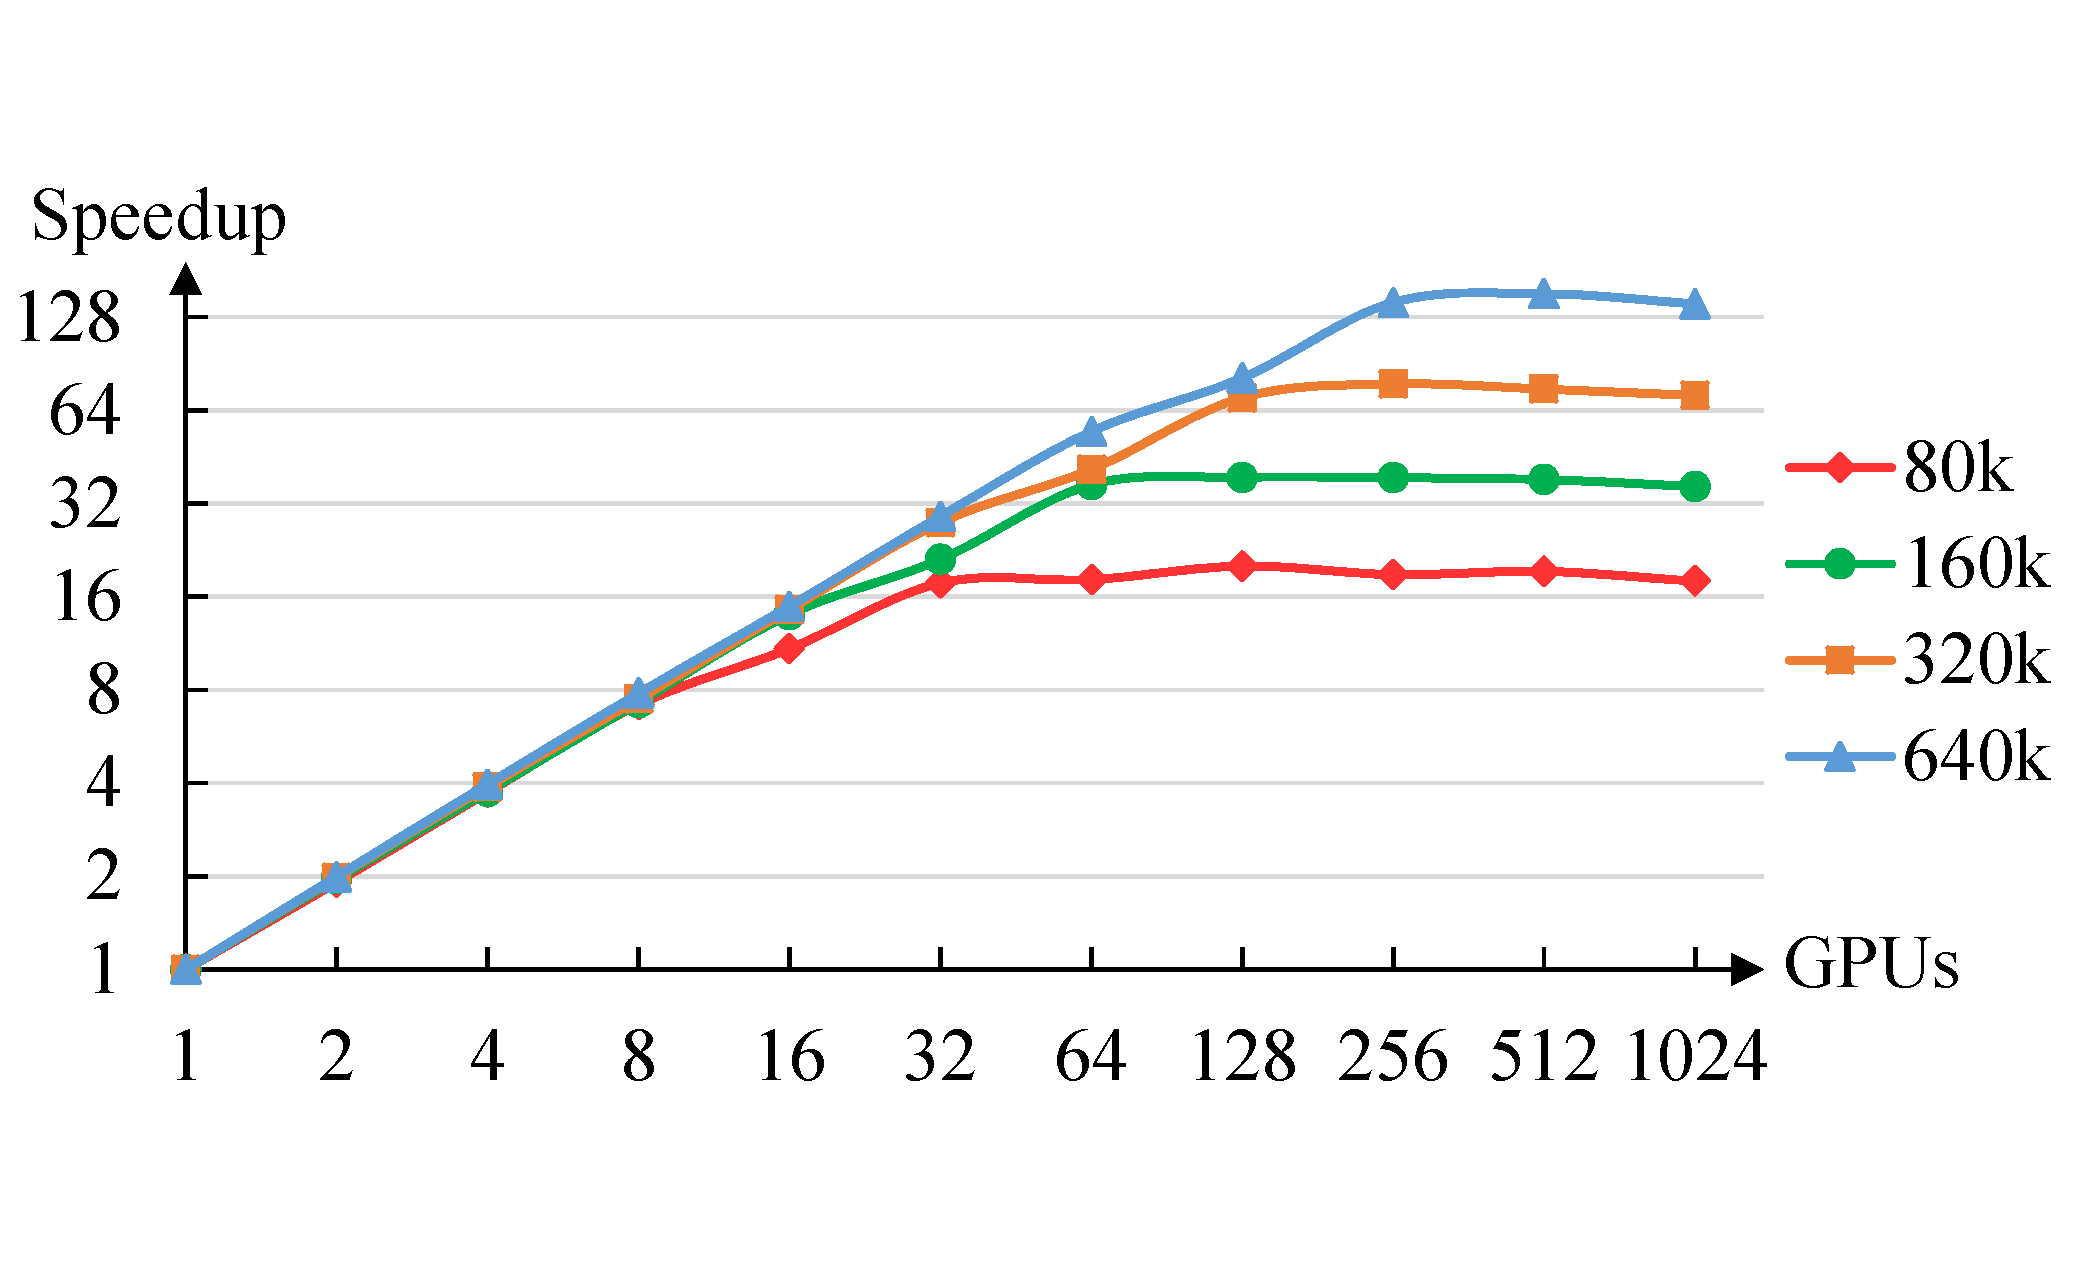
\includegraphics[width=\textwidth]{Img/640k_speedup_of_space_charge_kicker5log.pdf}
        \caption{空间电荷效应求解器加速比}
        \label{fig:SCTitan}
    \end{subfigure}
    \quad
    ~ %add desired spacing between images, e. g. ~, \quad, \qquad, \hfill etc.
      %(or a blank line to force the subfigure onto a new line)
    \begin{subfigure}[b]{0.9\textwidth}
        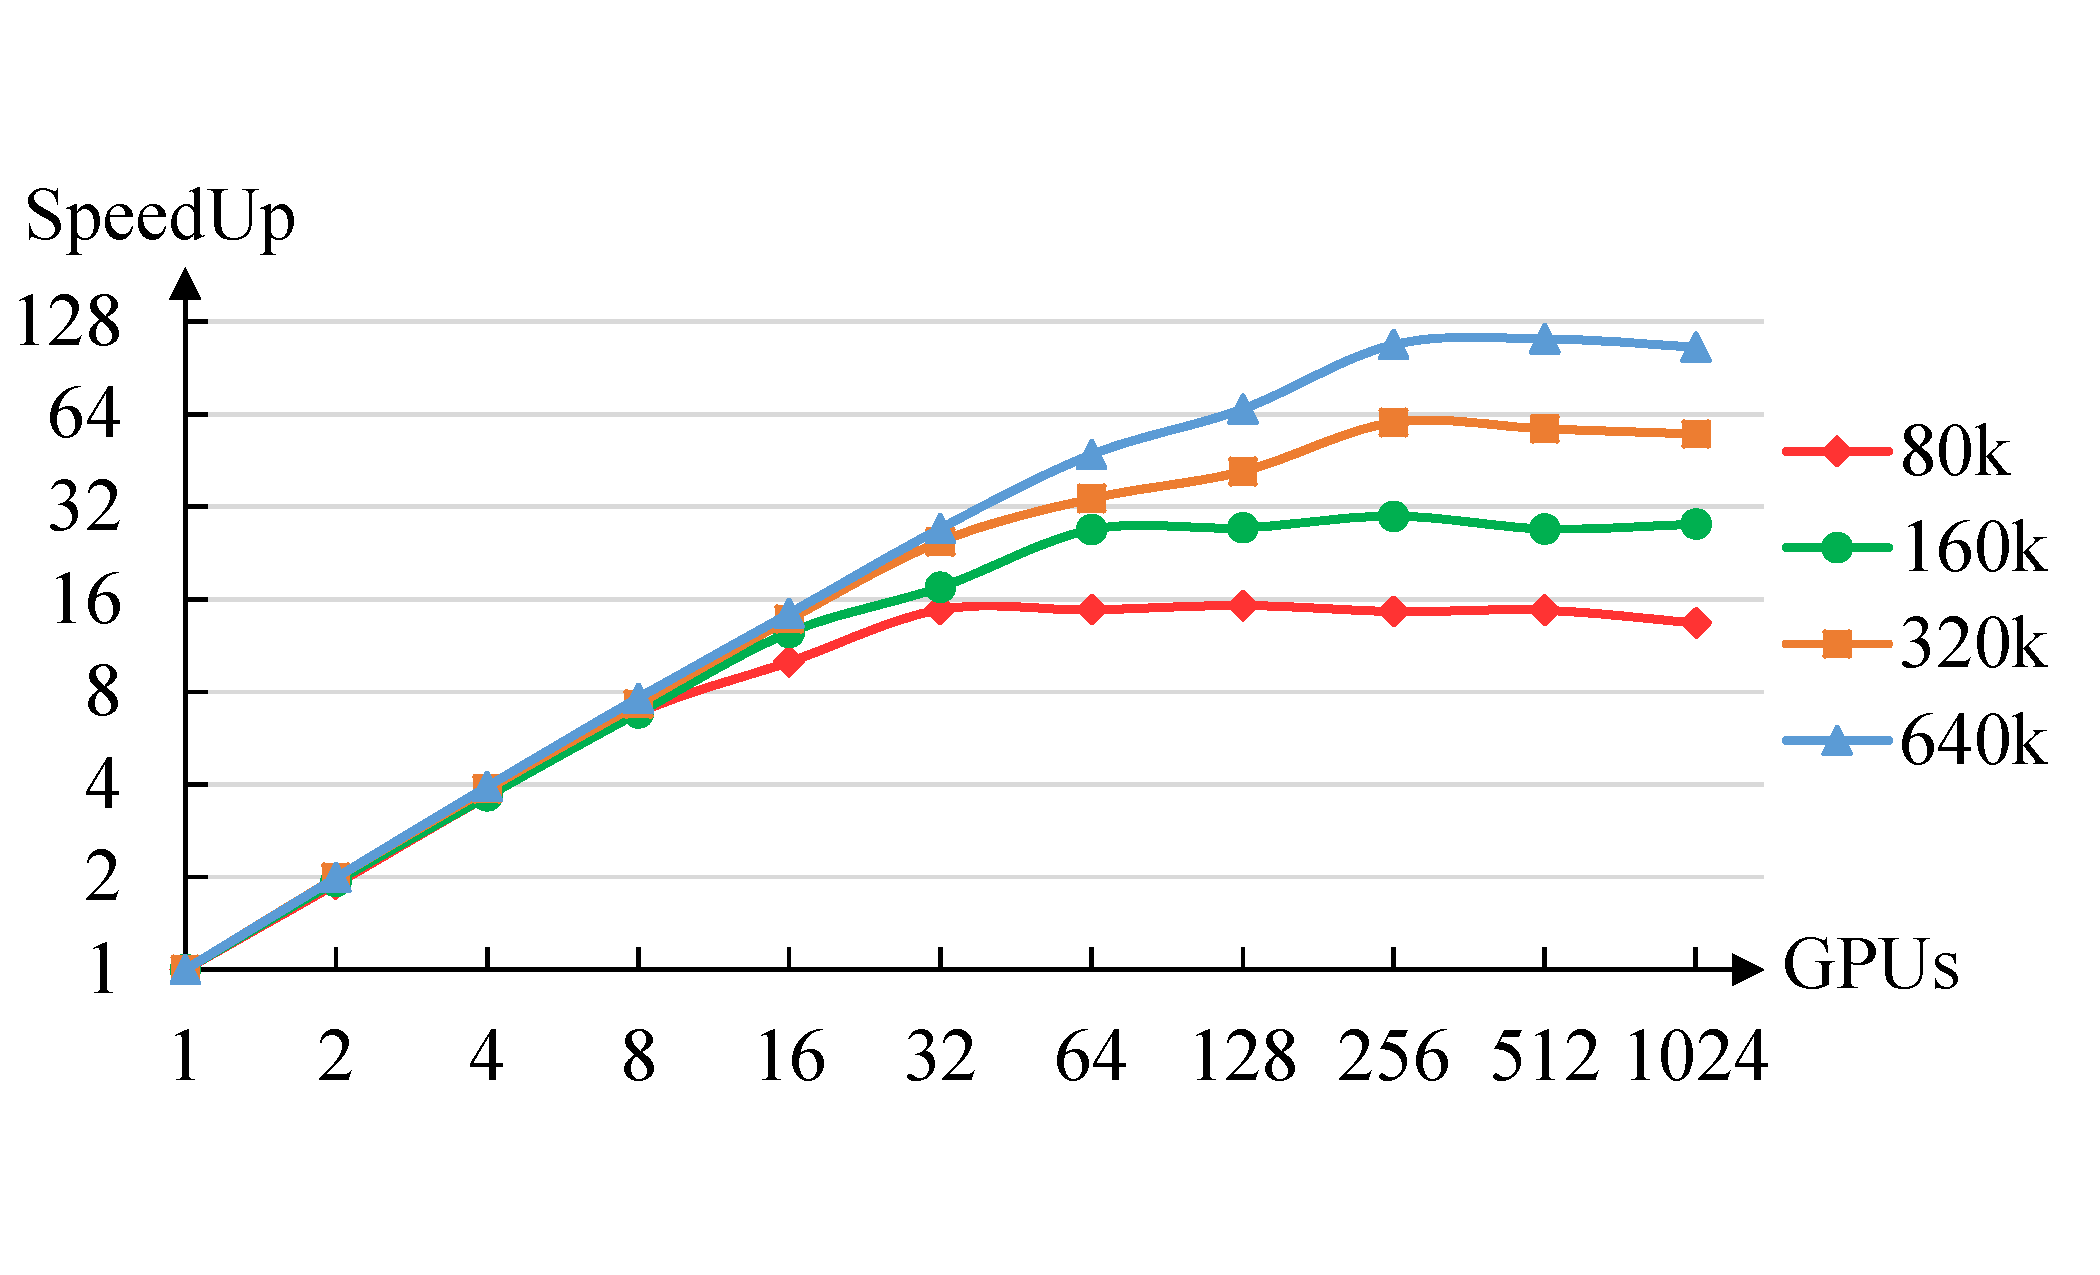
\includegraphics[width=\textwidth]{Img/640k_speedup_of_looptime5log.pdf}
        \caption{程序整体加速比}
        \label{fig:TotalTitan}
    \end{subfigure}
    \caption{多GPU加速比}\label{fig:Titan}
\end{figure}

由图\ref{fig:SCTitan}可得,在一开始,空间电荷效应求解器的加速比随着GPU的数目几乎线性增加,直到逐渐到达一个极限。
一方面,加速比的线性增长主要是因为GPU之间的数据交换量很少,导致通讯时间很少。
这是无网格Symplectic粒子跟踪算法的一个很大的优势,各个进程之间的数据交换量仅与阶数有关,而与粒子数量无关。
另一方面,它可以实现的最大加速度主要受粒子数量的限制,线性增加的范围和极限也随着粒子数量的增加而增加。
以160k粒子为例,加速比最大可以达到40。在Titan集群上,每个GPU包含2688个内核,
当使用64个GPU时,我们使用了64 $\times$ 2688 = 172032个内核,即使用的核心数大于粒子数。
在这种情况下,我们无法通过简单地使用更多的GPU来获得进一步加速。
而粒子数目增加时,比如320k个粒子或640k个粒子,所能够使用的GPU数目也会随之增加,最大加速比和线性范围也就会增加。

图\ref{fig:TotalTitan}是程序整体总时间的加速比,其中外部传输矩阵,坐标变换,粒子信息统计这些部分也是并行化的。
因为它们的计算量较低,很难取得很高的并行度。所以加速比略微下降。
但是因为其他部分在程序整体耗时中所占比重很小,所以下降幅度很小。

\section{小结}                      \label{section:Performance_conclusion}
通过对并行程序的性能测试可以看出,对于PIC算法,在单个普通家用GPU (GTX 1060) 上相对于单核CPU实现了超过50倍的加速。
当模拟使用的粒子数较大时,PIC算法在GPU集群上也显示出良好的可扩展性;而当粒子数目较小时其可扩展性较差。

对于Symplectic算法,在一个普通家用GPU上相对于单核CPU实现了超过450倍的加速比。
同时,我们在GPU集群Titan上的测试还显示出这种算法有良好的可扩展性,程序的加速比随着GPU数目几乎线性增加。
在未来的研究中,我们将继续扩展此模型速发,并在不同架构的计算机上比较Symplectic算法的效率。